\subsection{Обзор существующих алгоритмов}

Существует большое количество методов как генерации распределенных ансамблей, так и их анализа.

Под термином идеальная упаковка подразумевается такой вид упаковки, при котором изначально существует некоторая структурировать расположения элементов в пространстве, но затем вводя стохастику по каким-либо параметрам (допустим все присутствующие оси координат, либо радиус-вектор и углы его отклонения от каких-либо осей) а также перемешивание по данным стохастическим параметрам, мы можем получить упаковку элементов любой сложности. В теории перколяции, кроме узлов и связей, наиболее распространённым элементом является сфера, поэтому значительная часть алгоритмов сначала разрабатывается для сфер, как для самых простых в изучении (и моделировании) форм.

Рассмотрим некоторые из реализованных алгоритмов построения случайно распределенных ансамблей сфер(как начинающих из изеальных упаковок так и обыкновенных):

\begin{enumerate}
    \item \label{meth:random_based}
    \textbf{Случайное расположение элементов} 
    \newline
    Алгоритм случайного расположения элементов является самым примитивным среди всех методов генерации случайного ансамбля. В его основе заложено большое количество попыток расположения элементов в пространстве до того момента, пока не получится случайным образом расположить элементы на заданном заранее пространстве.\newline
    Алгоритм:
    \begin{enumerate}[label=\arabic*)]
        \item 
        Случайным образом выбираются координаты внутри области, которую необходимо заполнить
        \item 
        Если при попытке расположения сферы заданного радиуса в данных выбранных координатах не возникает пересечений с другими сферами
        $$dist(circle[i],circle[j])<  2 \cdot circle\_radius, \forall i \neq j$$ то координаты центра данной сферы добавляются в массив всех сфер
        \item 
        Если за $max\_iteration\_count$ итераций расположения точки на пространстве  не набирается достаточное количество  непересекающихся сфер, то попытка начинается новая попытка. Это делается потому, что возможны такие расположения сфер в пространстве, при котором добавить дополнительные сферы невозможно, хотя их смещени позволило-бы добавить ещё сфер.
        \item 
        Если за определенное количество попыток $max\_attempt\_count$ расположения сфер (по $max\_iteration\_count$ итераций в каждой попытке), то расположение сфер считается неудавшимся. Данный подход используется потому, что такая ситуация возможна, когда пользователю необходимо расположить сферы по плотности близко, к плотнейшей упаковке, а добиться такого расположения случайным выбором координат крайне маловероятное событие. 
    \end{enumerate}
    Недостатком данного подхода является выраженный порог плотности заполнения, после которого сложность размещения каждой следующей сферы значительно растёт (подробнее будет рассмотрено в разделе \ref{tesing}).
    \newcommand{\imgsize}{6cm}
    \begin{figure}[h!]
        \begin{subfigure}{0.49\textwidth}
            \centering
            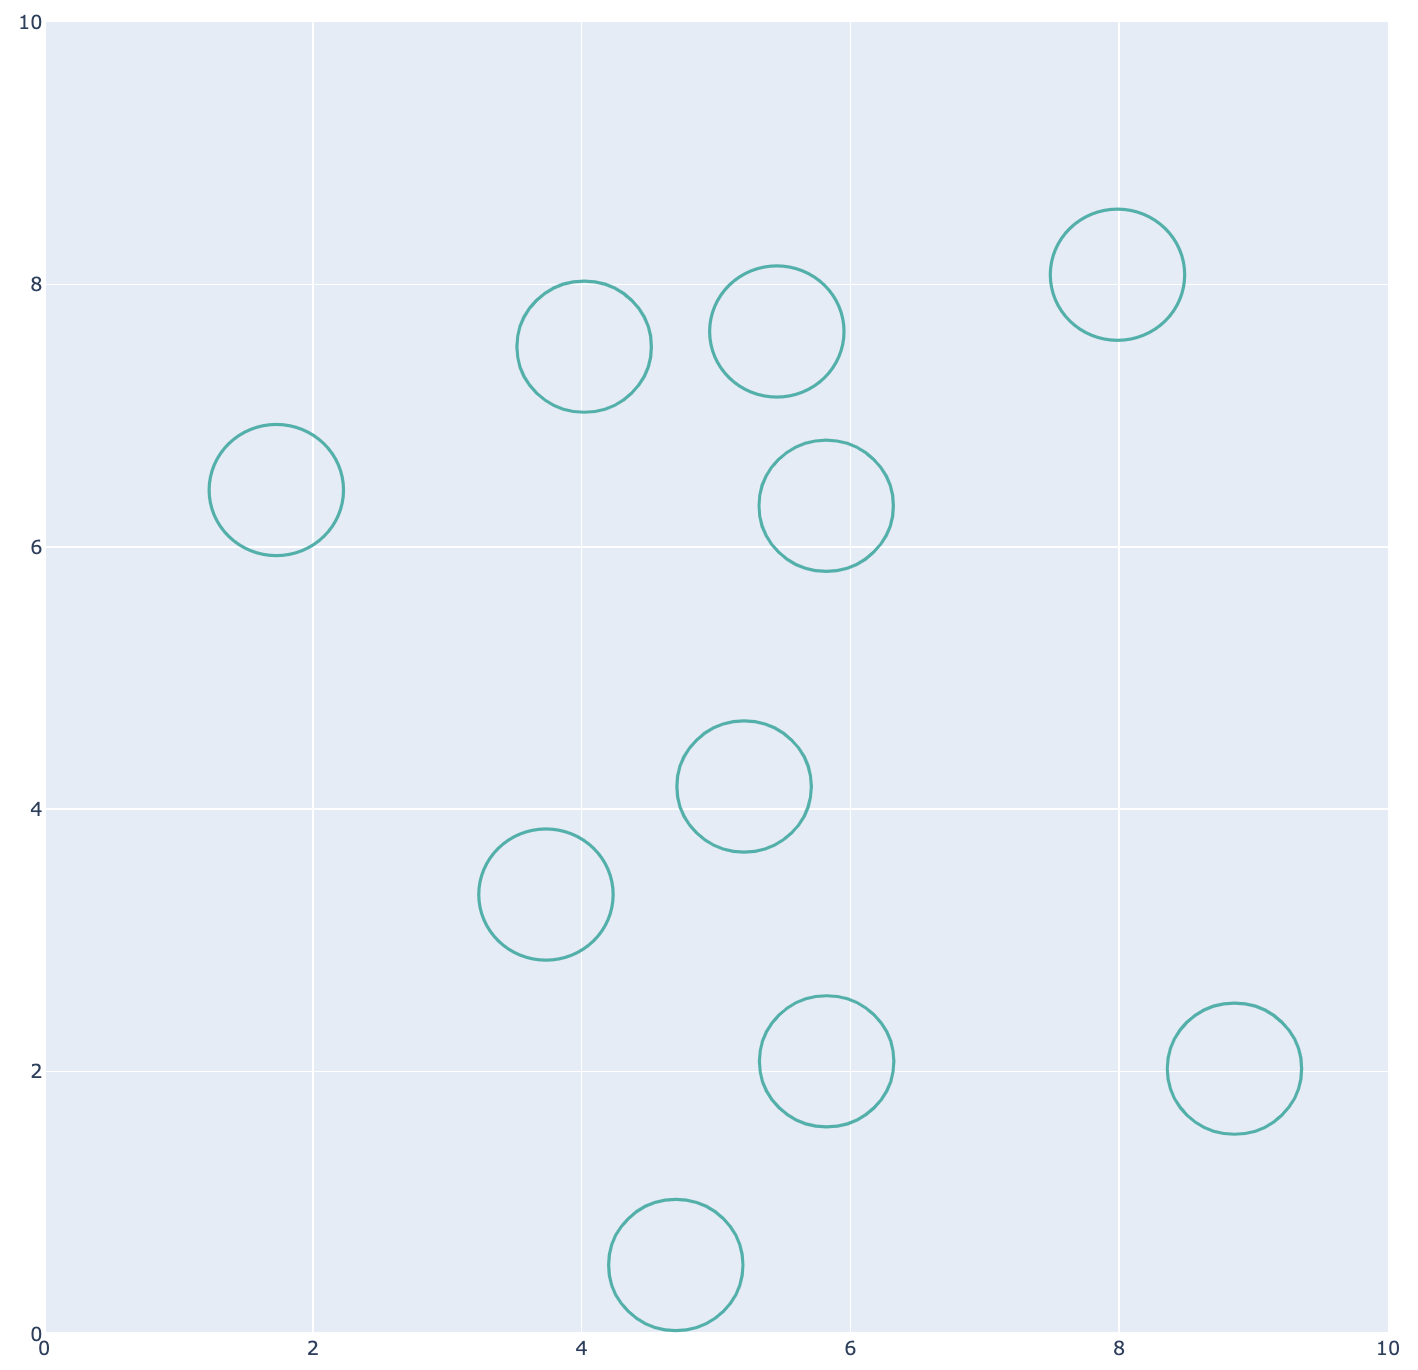
\includegraphics [width=\imgsize,height=\imgsize]{figures/rand_pack/c10att1iter12totiter12.png}
            \caption{Шаров: $10$, попытка: $1$, итераций: $12$}
        \end{subfigure}
        \begin{subfigure}{0.49\textwidth}
            \centering
            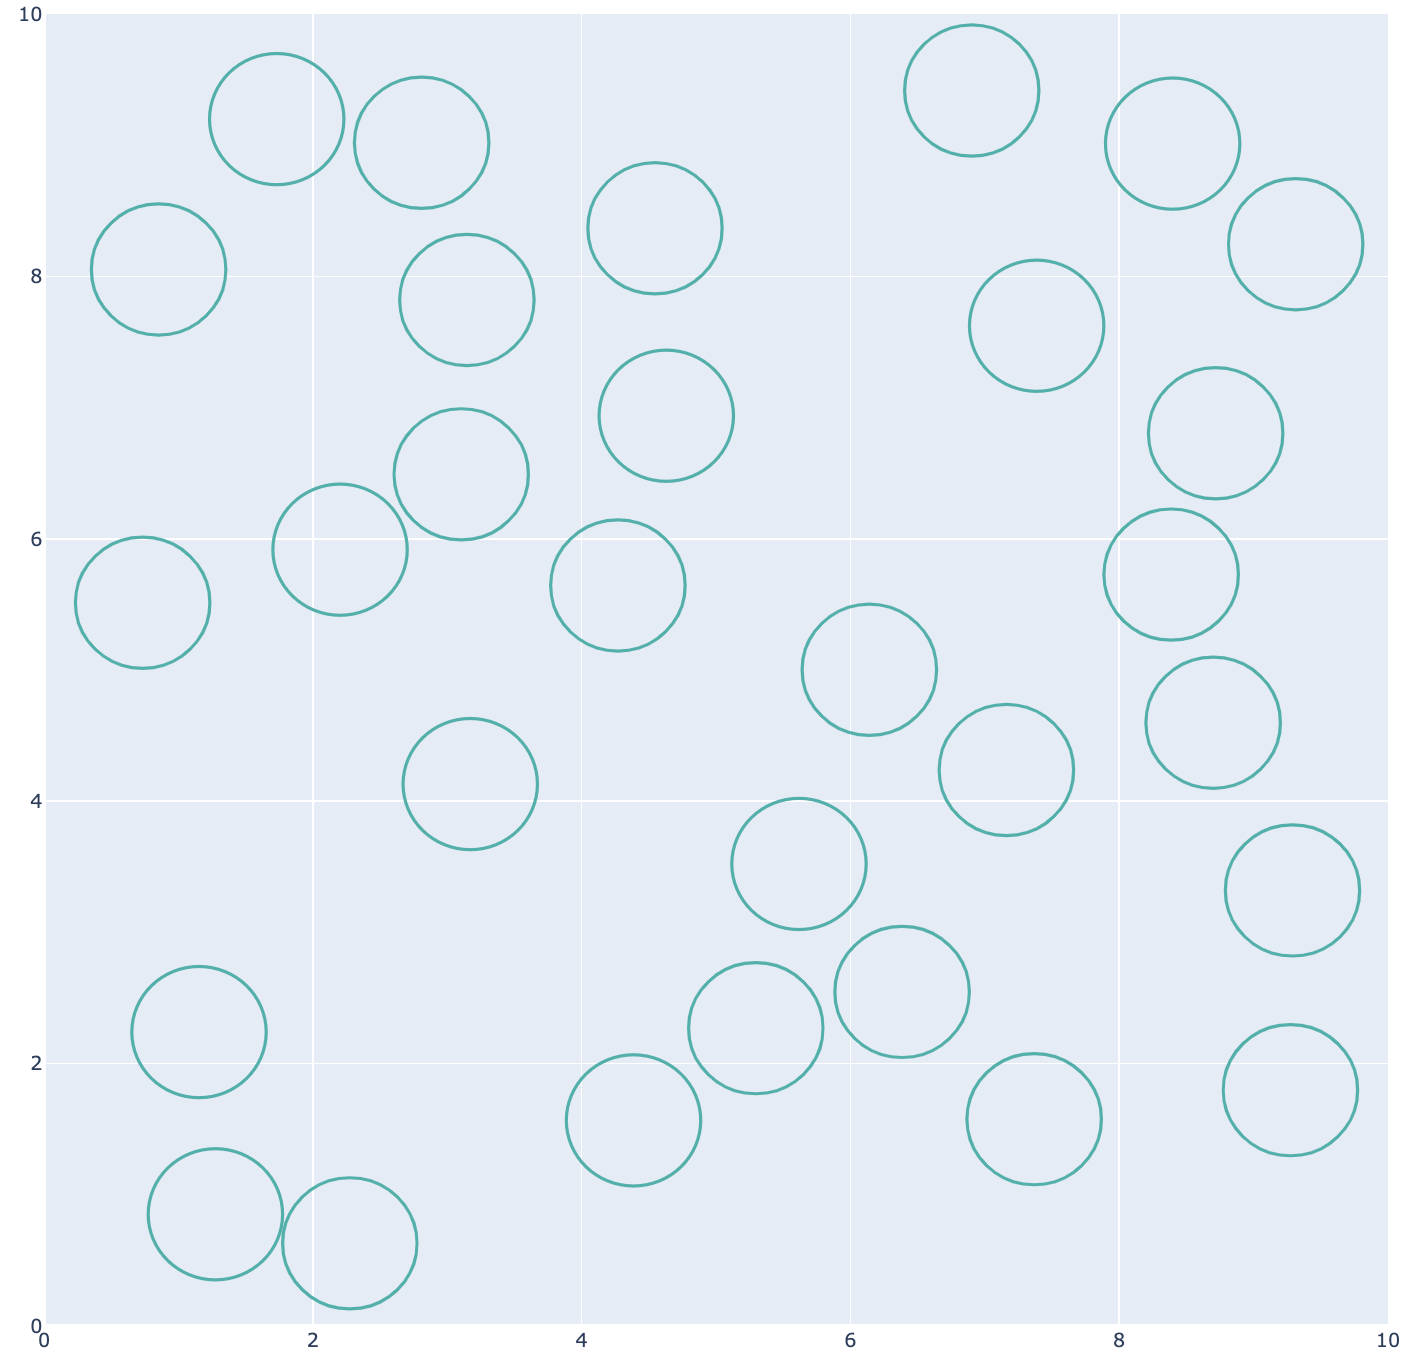
\includegraphics [width=\imgsize,height=\imgsize]{figures/rand_pack/c30att1iter42totiter42.png}
            \caption{Шаров: $30$, попытка: $1$, итераций: $42$}
        \end{subfigure}
        \begin{subfigure}{0.49\textwidth}
            \centering
            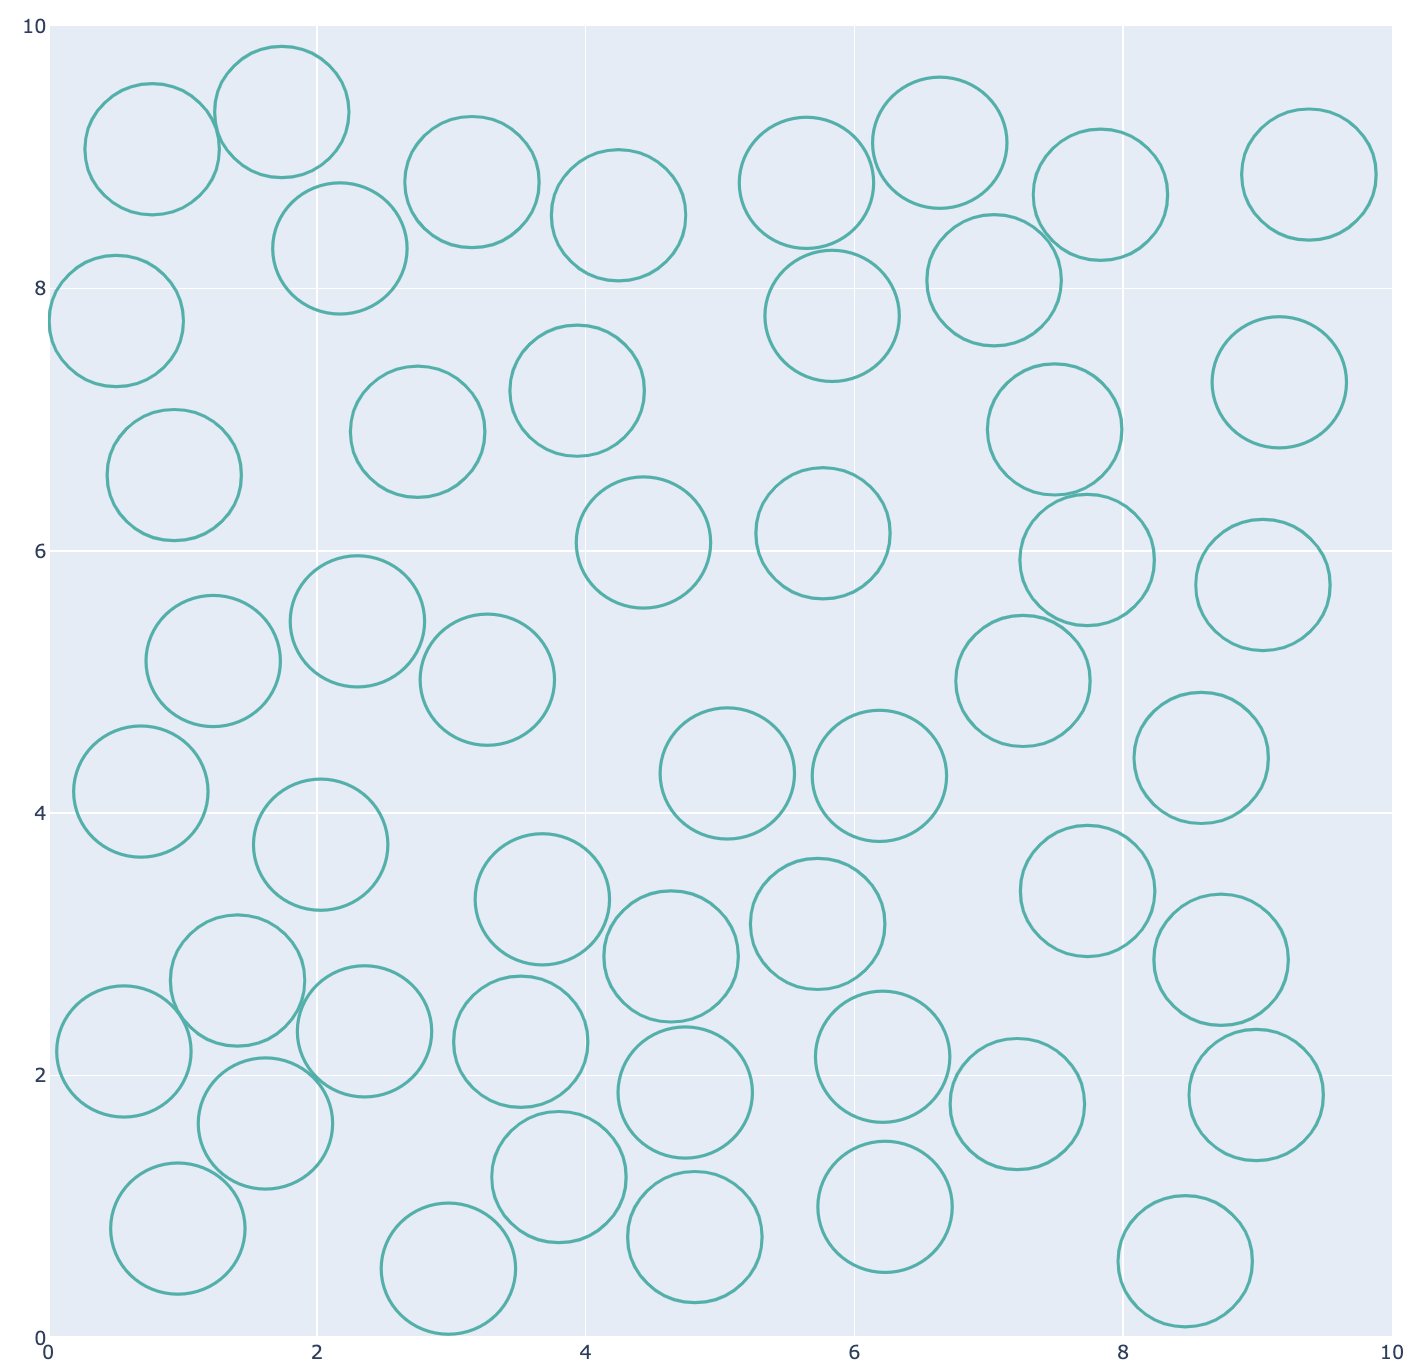
\includegraphics [width=\imgsize,height=\imgsize]{figures/rand_pack/c50att1iter629totiter629.png}
            \caption{Шаров: $50$, попытка: $1$, итераций: $629$}
        \end{subfigure}
        \begin{subfigure}{0.49\textwidth}
            \centering
            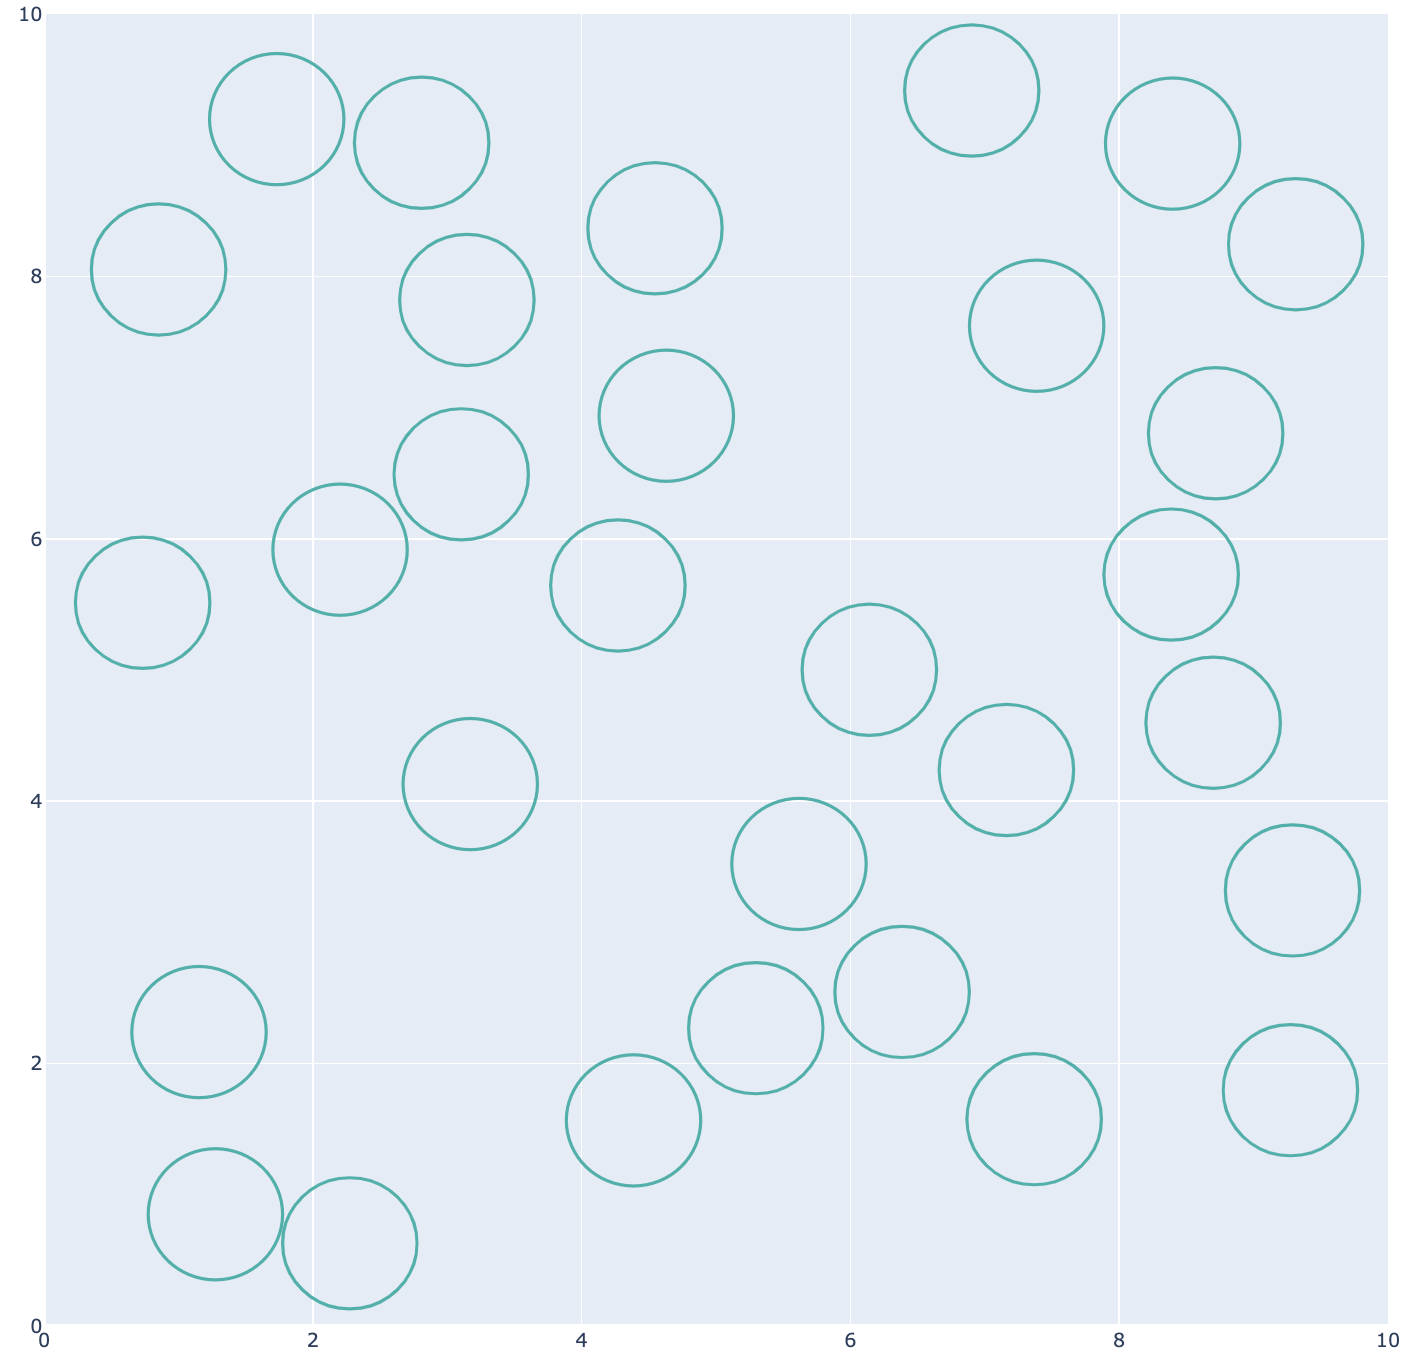
\includegraphics [width=\imgsize,height=\imgsize]{figures/rand_pack/c30att1iter42totiter42.png}
            \caption{Шаров: $65$, попытка: $3$, итераций: $29219$}
        \end{subfigure}
        \caption{Расположение шаров}
    \end{figure}
    \begin{figure}[h]
        \centering
        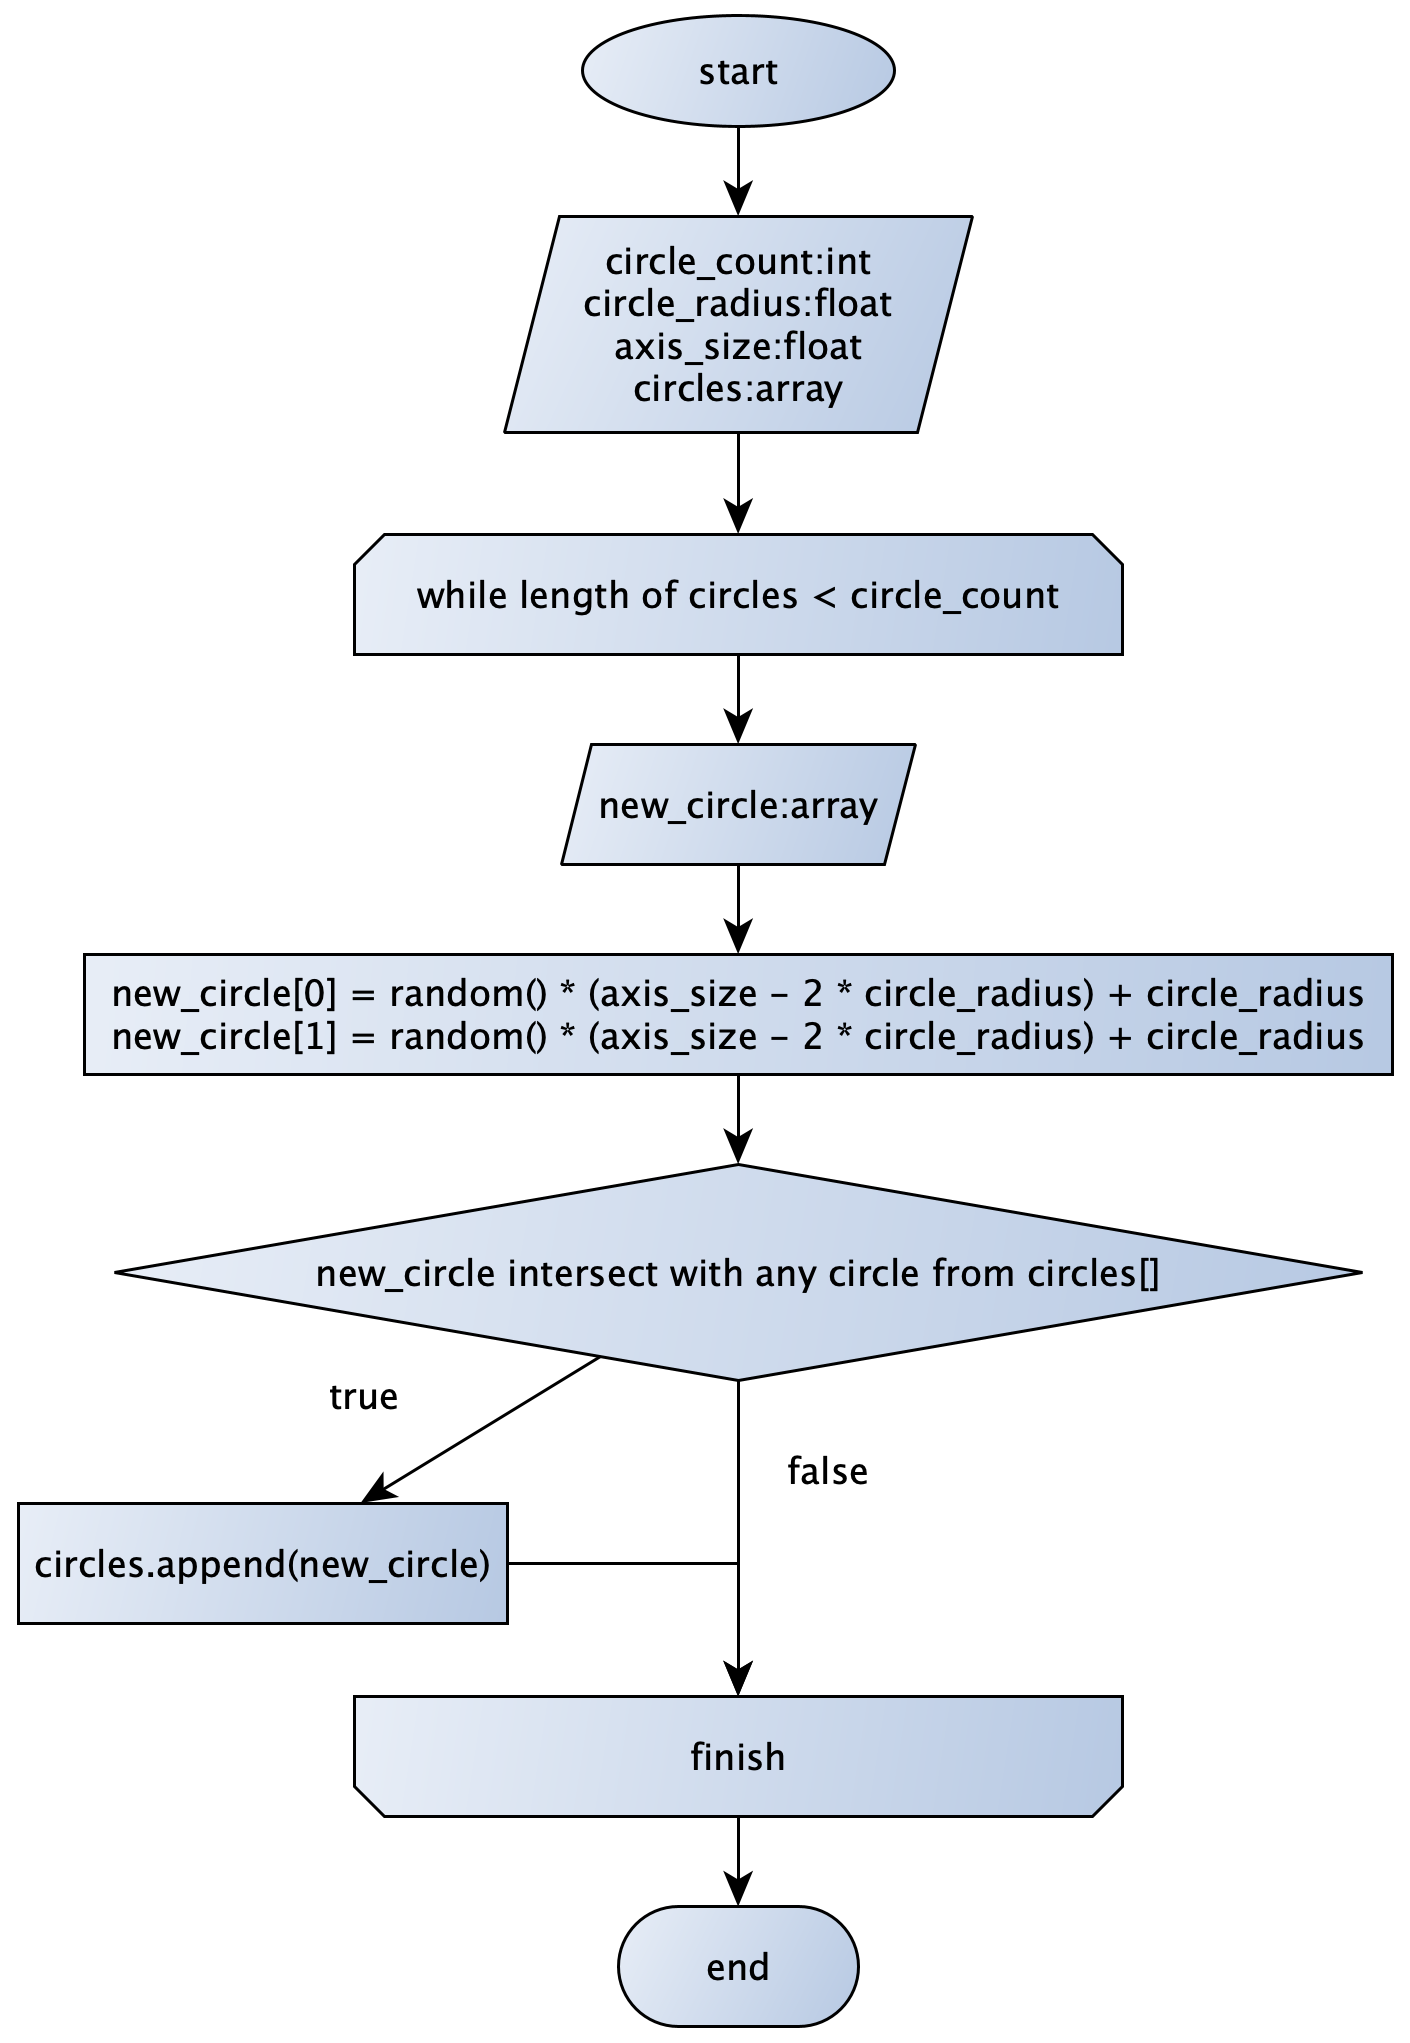
\includegraphics
        [width=10cm,height=15cm]
        {figures/rand_pack/random_circles.png}
        \caption{Блок-схема случайного расположения элементов}
        \label{fig:my_label}
    \end{figure}
    \item \label{meth:mesh_based}
    \textbf{Метод, основанный на сетке}\newline 
    Данный метод можно отнести к классу методов начинающих из идеального расположения элементов. Суть данного метода заключается в том, чтобы сначала с возможным избытком расположить элементы в квадратную сетку, а затем из этого возможно избыточного множества выбрать первые $circle\_count$ окружностей/сфер.\newline
    Алгоритм:
    \begin{enumerate}[label=\arabic*)]
        \item 
        Определить следующий полный квадрат $perfect\_square$ после количества окружностей $circle\_count$, которые необходимо расположить, и его корень \newline $perfect\_square\_root$.
        \item 
        Создать сетку из ячеек в $perfect\_square\_root \times perfect\_square\_root$ равномерно распределенную по пространству. Шаг сетки: 
        $$
        dl=a/perfect\_square\_root
        $$ 
        где $a$ - размер пространства в котором располагаются шары.
        \item
        Из заполненной сетки случайным образом выбрать $circle\_count$ окружностей.
        \item
        Перемешать выбранные сферы на плоскости.
    \end{enumerate}
    Как результат такого действия, мы получаем ансамбль случайно распределенных окружностей. Если при использовании метода (\ref{meth:random_based}) уже после расположения 60 шаров возникали трудности, то для того-же пространства метод (\ref{meth:mesh_based}) без проблем расположил и 70 и 80 шаров. Это показывает, что подход с идеальным начальным расположением шаров даёт значительное преимущество как по заполнению пространства так и по скорости работы, ведь не нужно перебирать бесконечное множество вариантов расположения для шара, а достаточно выбирать сразу среди доступных.
    \renewcommand{\imgsize}{7cm}
    \begin{figure}[h!]
        \begin{subfigure}{0.49\textwidth}
            \centering
            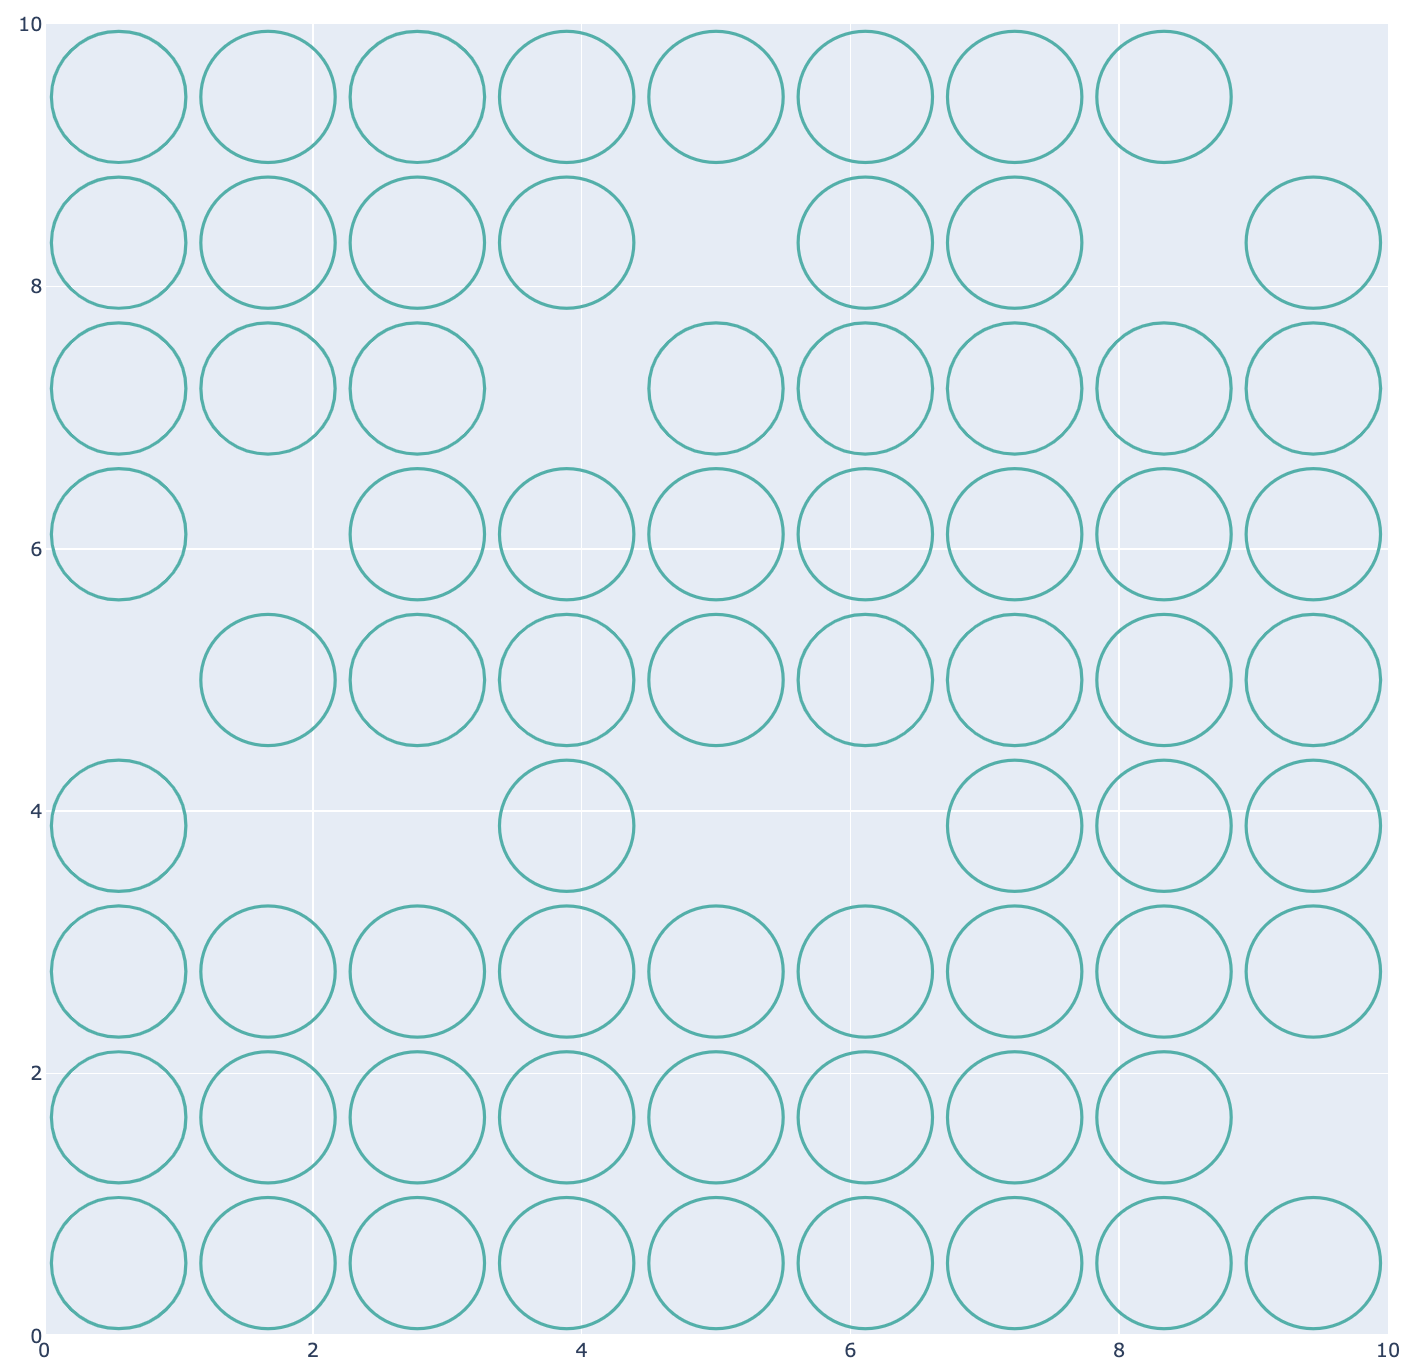
\includegraphics [width=\imgsize,height=\imgsize]{figures/mesh_based/70_before_shuffeling.png}
            \caption{Шаров $70$, до перемешивания}
        \end{subfigure}
        \begin{subfigure}{0.49\textwidth}
            \centering
            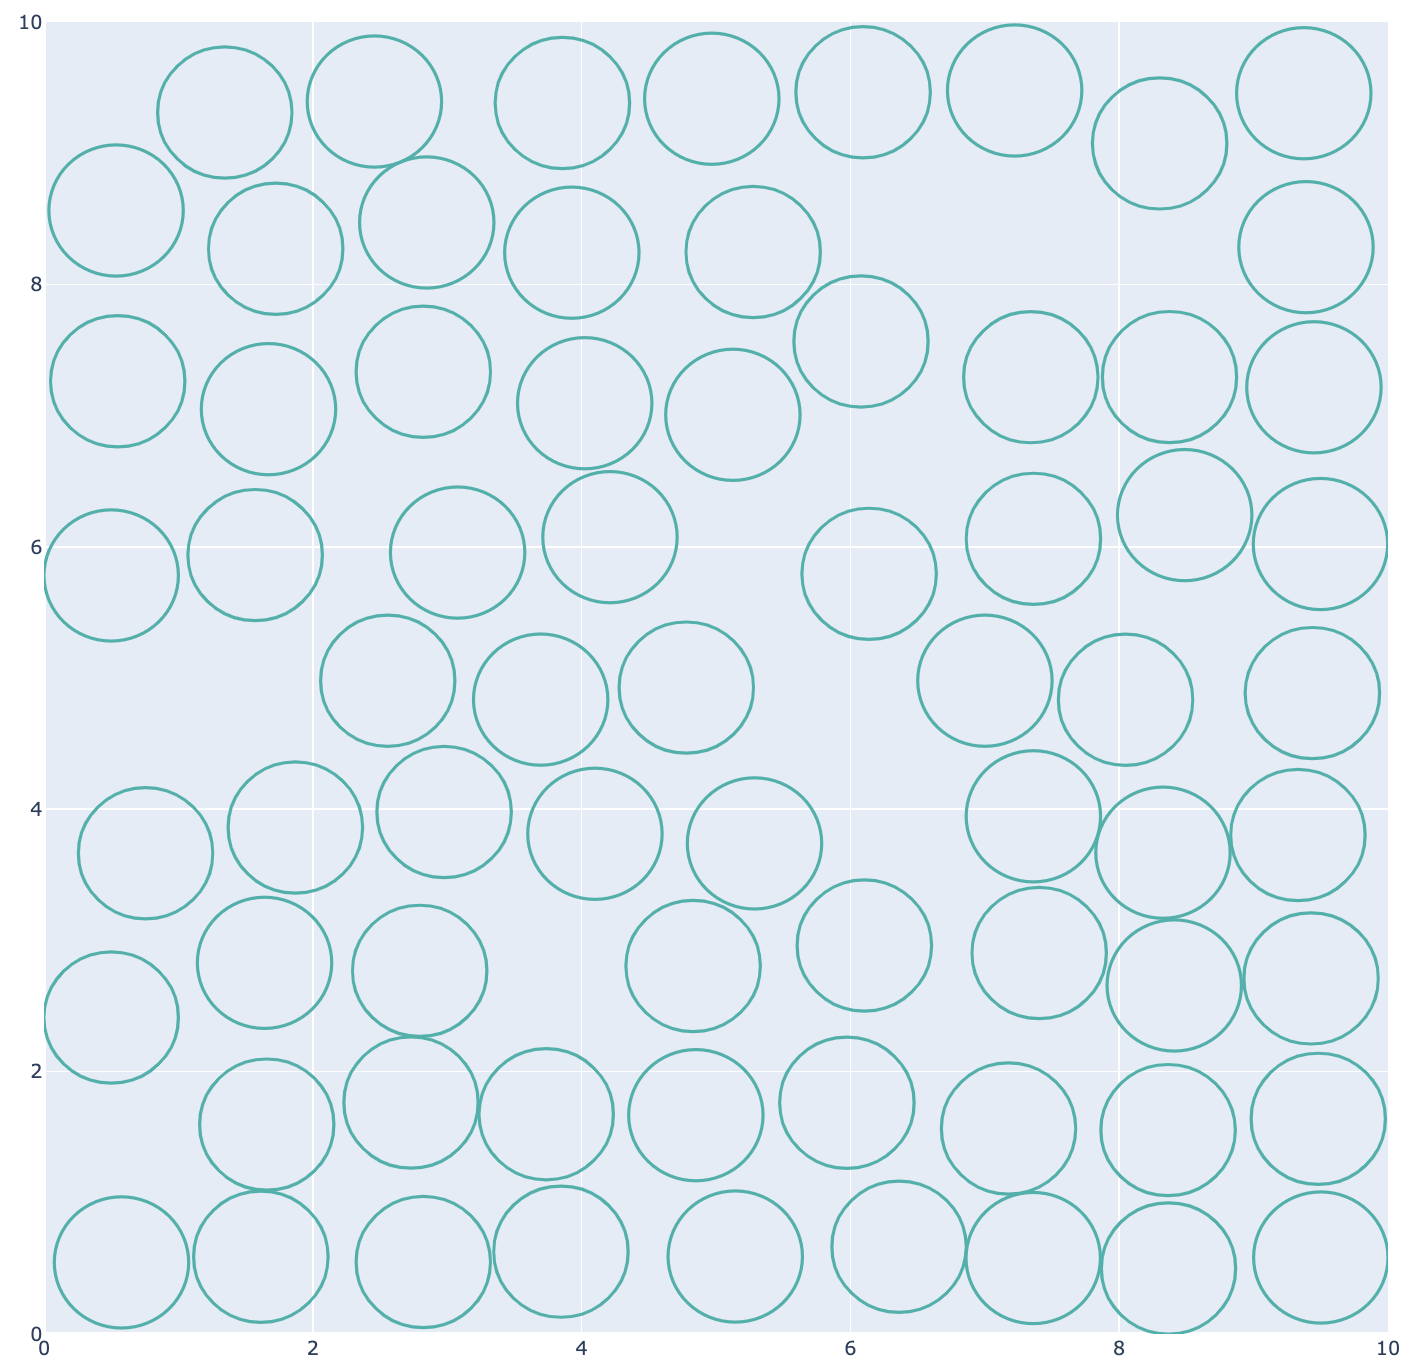
\includegraphics [width=\imgsize,height=\imgsize]{figures/mesh_based/70_after_shuffeling.png}
            \caption{Шаров $70$, до перемешивания}
        \end{subfigure}
        \begin{subfigure}{0.49\textwidth}
            \centering
            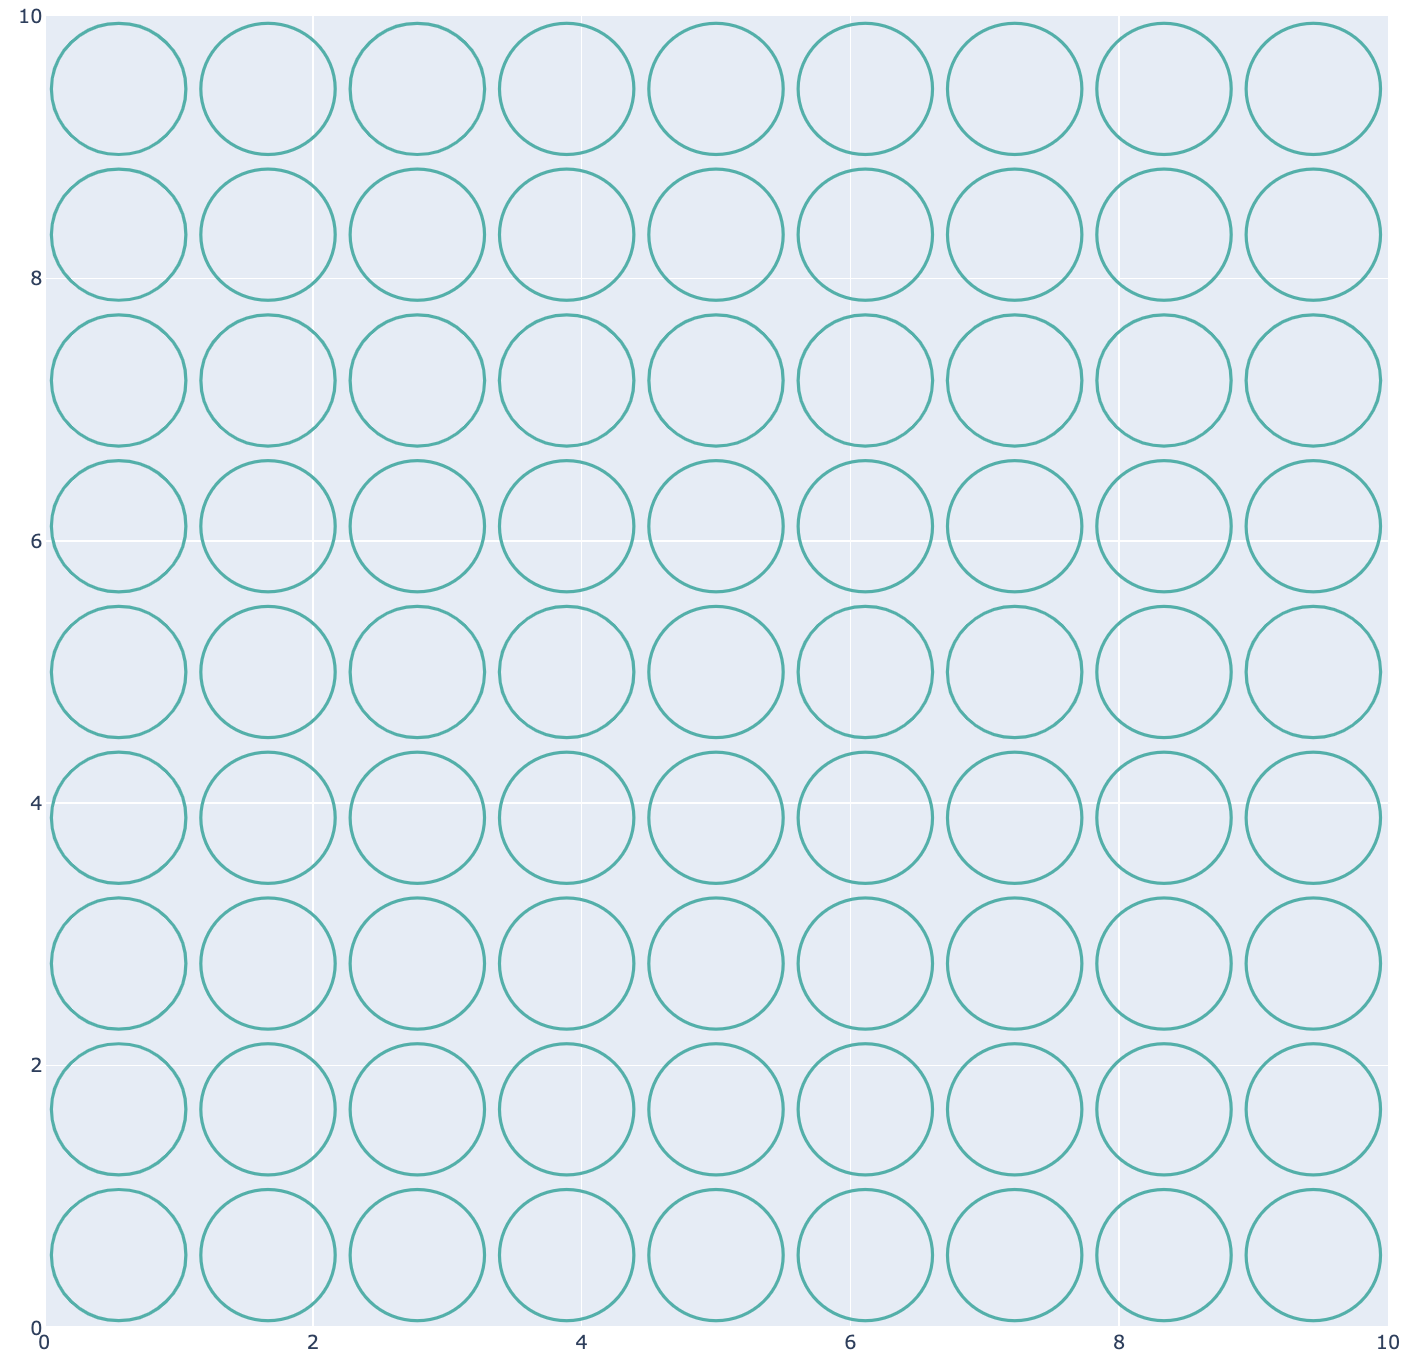
\includegraphics [width=\imgsize,height=\imgsize]{figures/mesh_based/81_before_shuffeling.png}
            \caption{Шаров $81$, до перемешивания}
        \end{subfigure}
        \begin{subfigure}{0.49\textwidth}
            \centering
            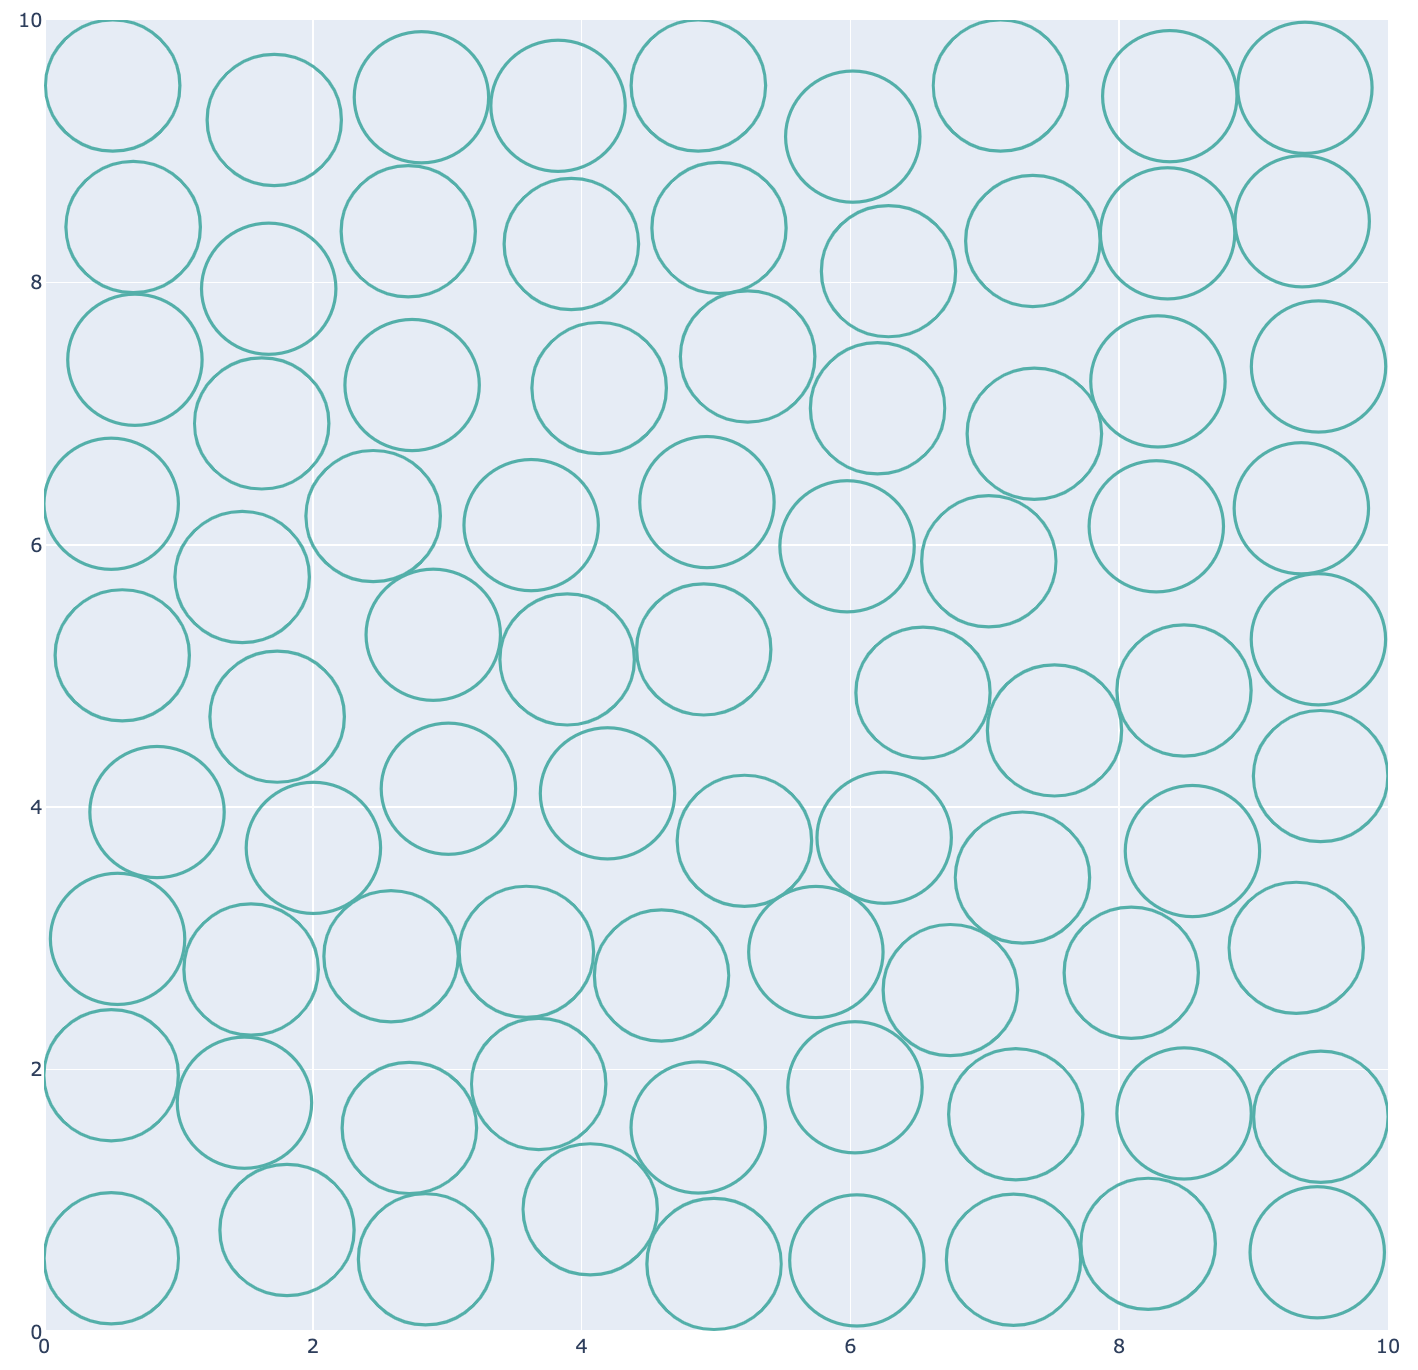
\includegraphics [width=\imgsize,height=\imgsize]{figures/mesh_based/81_after_shuffeling.png}
            \caption{Шаров $81$, после перемешивания}
        \end{subfigure}
        \caption{Расположение шаров}
    \end{figure}
    \begin{figure}[h!]
        \centering
        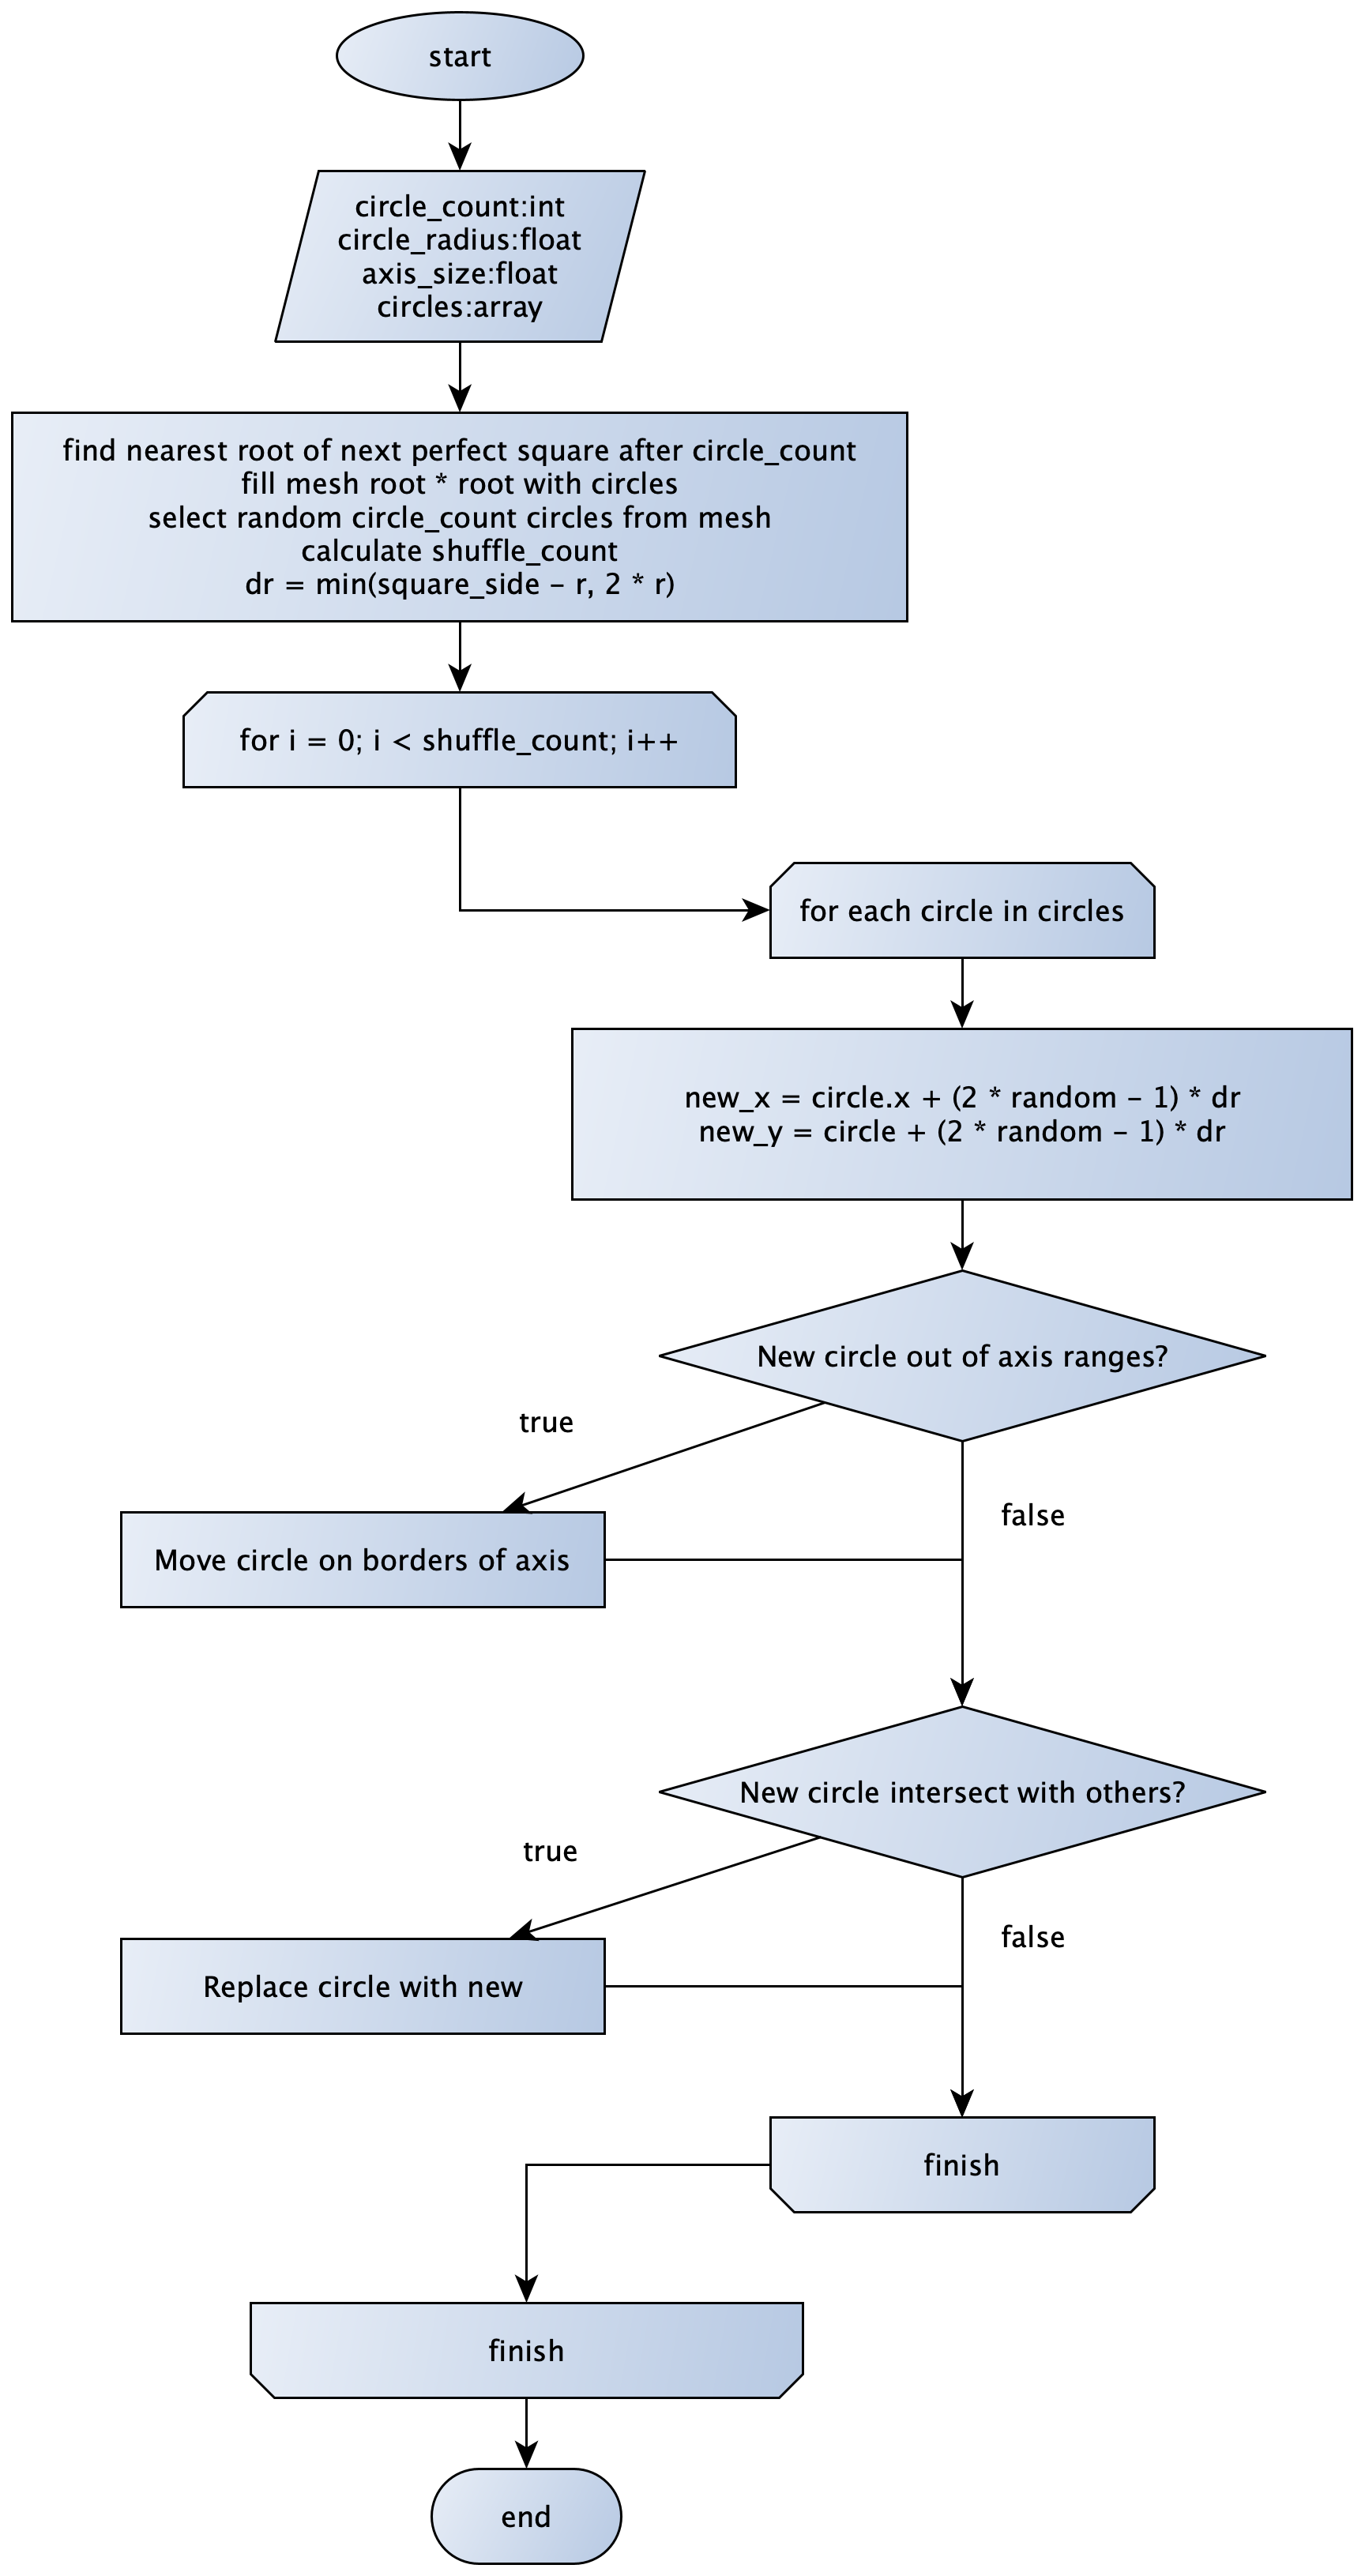
\includegraphics
        [width=15cm,height=20cm]
        {figures/mesh_based/mesh_based_circles.png}
        \caption{Блок-схема расположения основанного на сетке}
        \label{fig:my_label}
    \end{figure}
    \newpage
    \item 
    \textbf{Метод основанный на плотнейшей упаковке} \newline
    Данный метод позволяет добиться максимальной упаковки окружностей на площади. Для того, чтобы увеличить максимальную плотность возможного расположения сфер на площади, следует прибегнуть к плотнейшим упаковкам (раздел \ref{subsubsect:tight_packing}). \newline
    Алгоритм:
    \begin{enumerate}[label=\arabic*)]
        \item 
        Определить следующий полный квадрат $perfect\_square$ после количества окружностей $circle\_count$, которые необходимо расположить, и его корень \newline $perfect\_square\_root$.
        \item 
        Создать сетку из ячеек в $perfect\_square\_root \times perfect\_square\_root$ распределенную по пространству методом плотнейшей упаковки.
        \item
        Растянуть все сферы на полное пространство.
        \item
        Перемешать выбранные сферы на плоскости.
    \end{enumerate}
    
    \renewcommand{\imgsize}{8cm}
    \newcommand{\imgsubdir}{tight_packing}
    \begin{figure}[h!]
        \begin{subfigure}{0.49\textwidth}
            \centering
            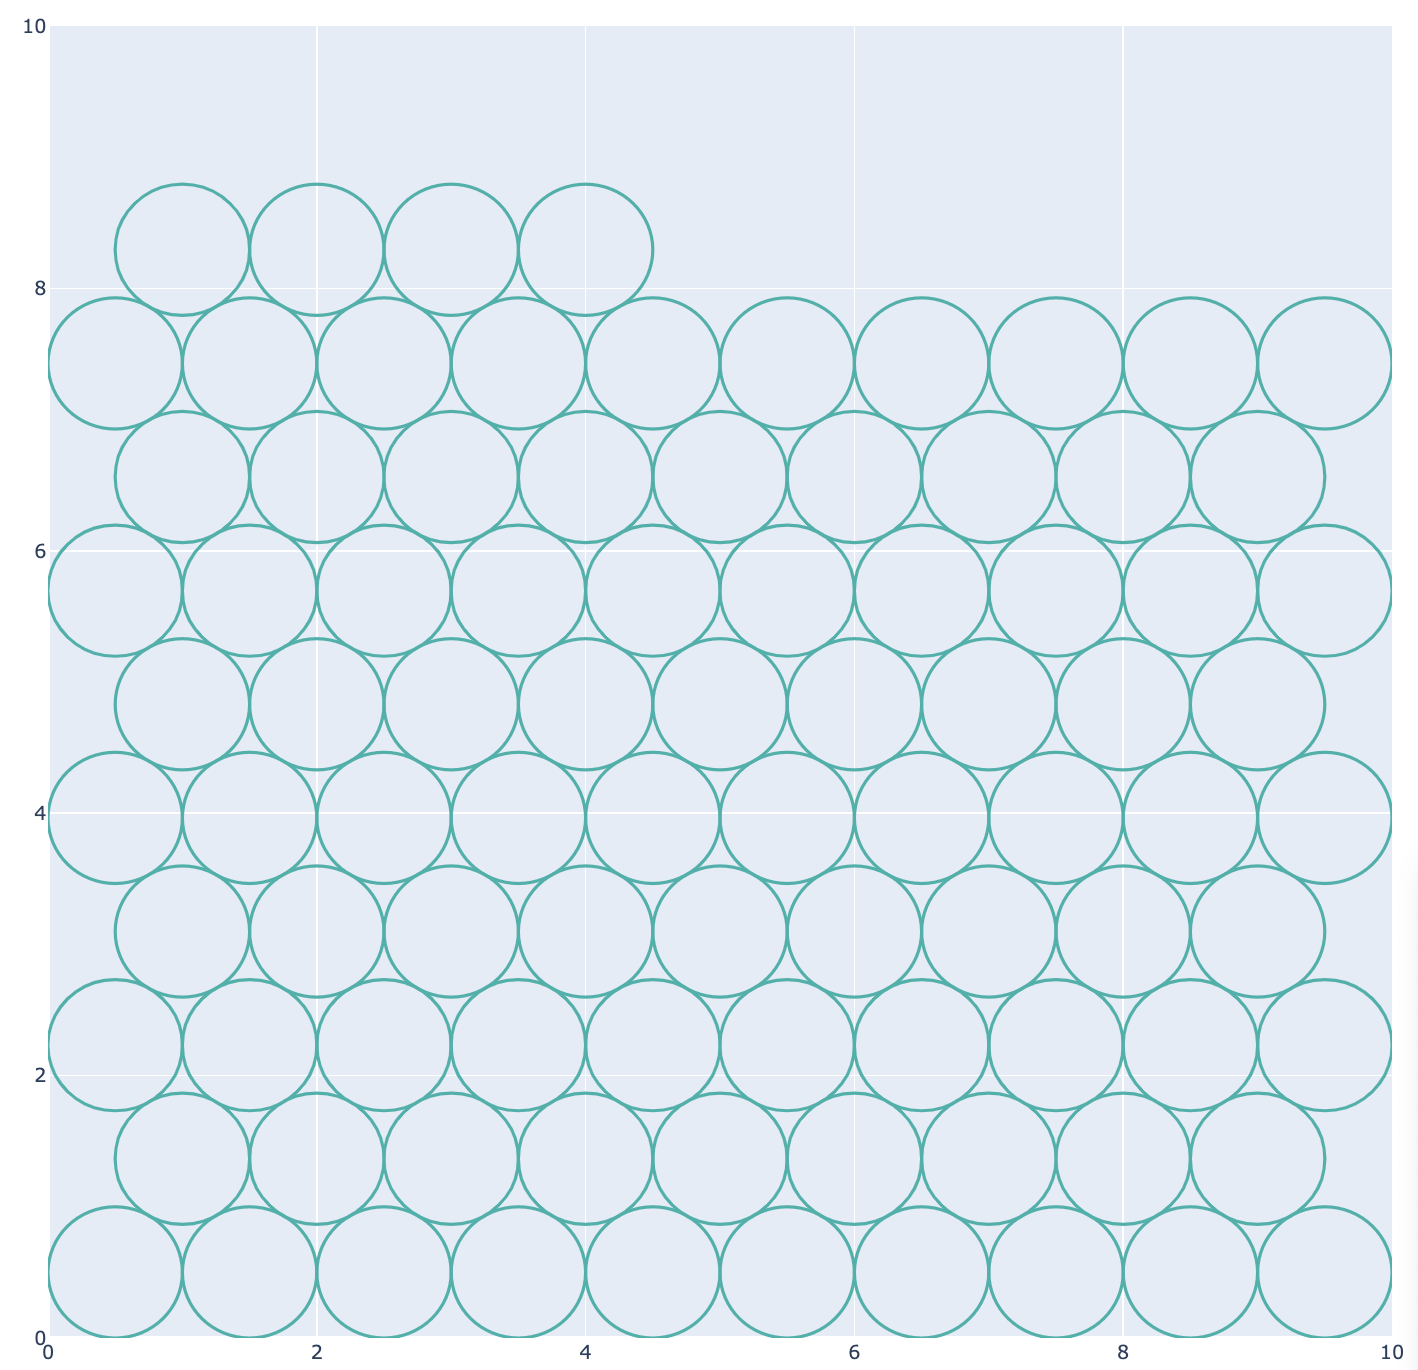
\includegraphics [width=\imgsize,height=\imgsize]
            {figures/\imgsubdir/90_packing.png}
            \caption{Шаров $90$, до перемешивания}
        \end{subfigure}
        \begin{subfigure}{0.49\textwidth}
            \centering
            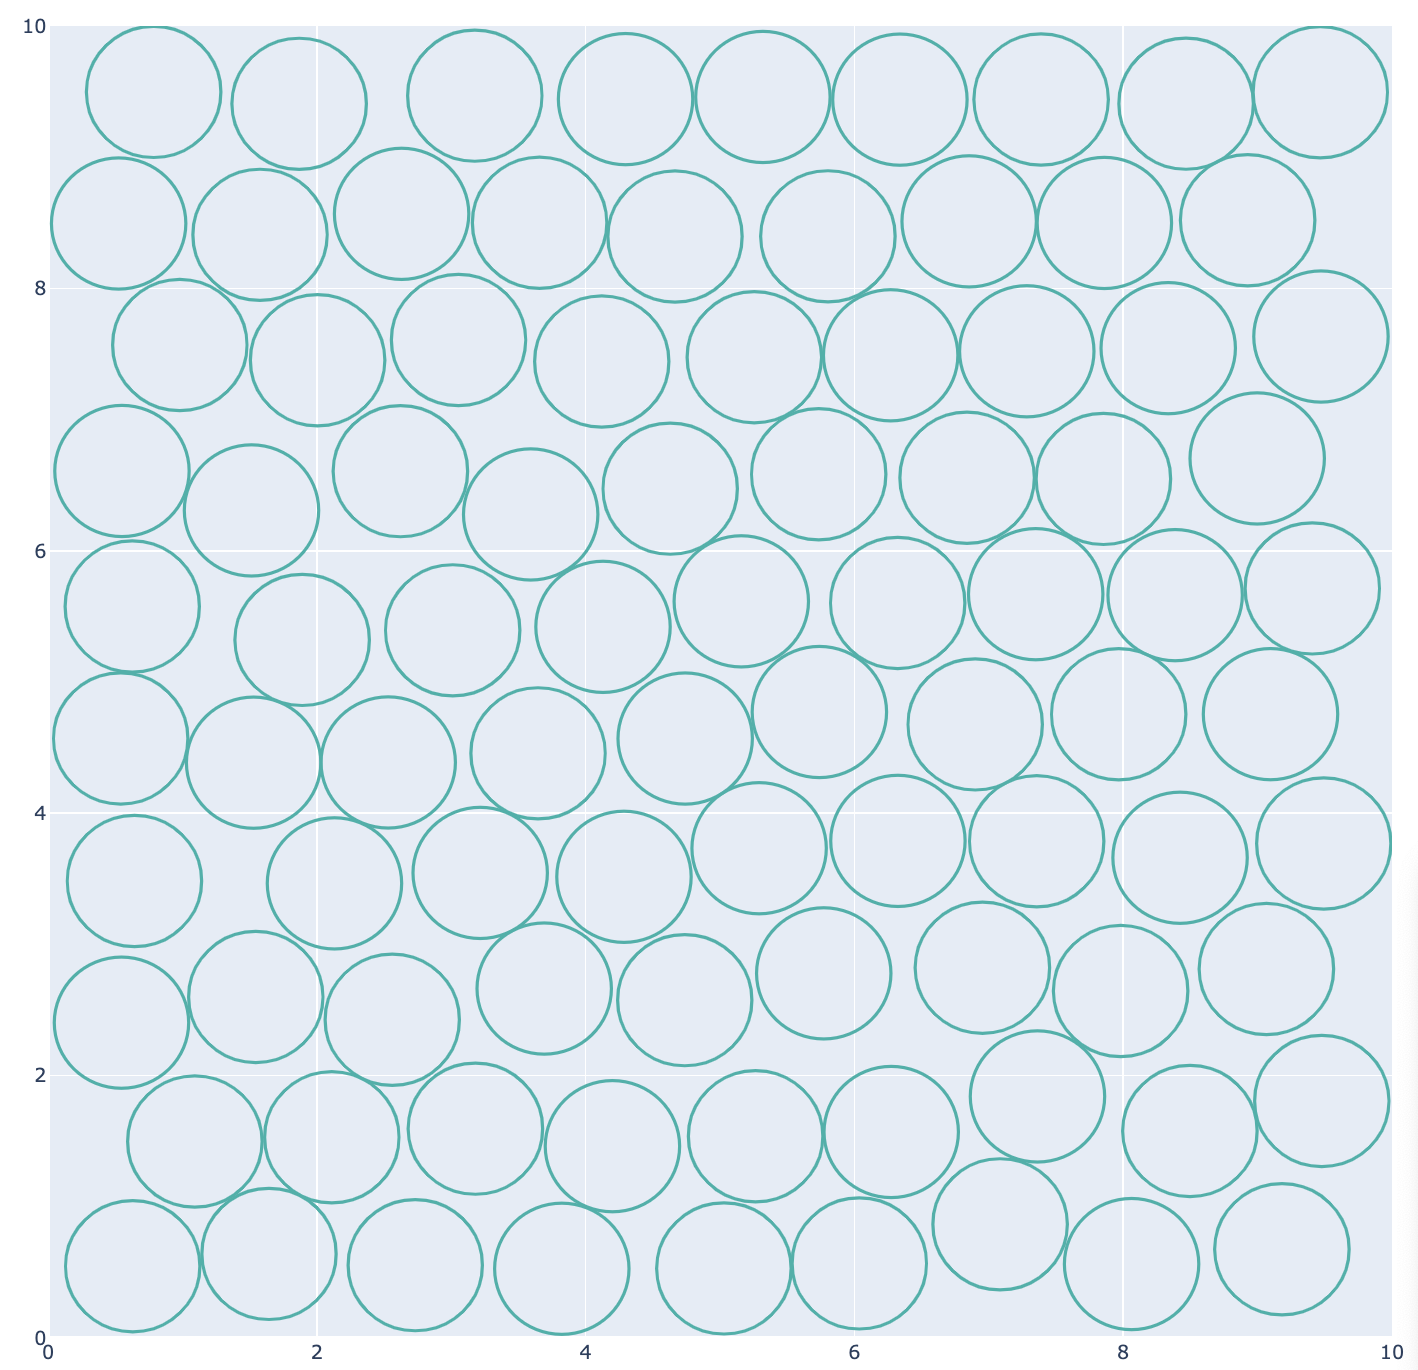
\includegraphics [width=\imgsize,height=\imgsize]
            {figures/\imgsubdir/90_shuffeling.png}
            \caption{Шаров $90$, после перемешивания}
        \end{subfigure}
        \begin{subfigure}{0.49\textwidth}
            \centering
            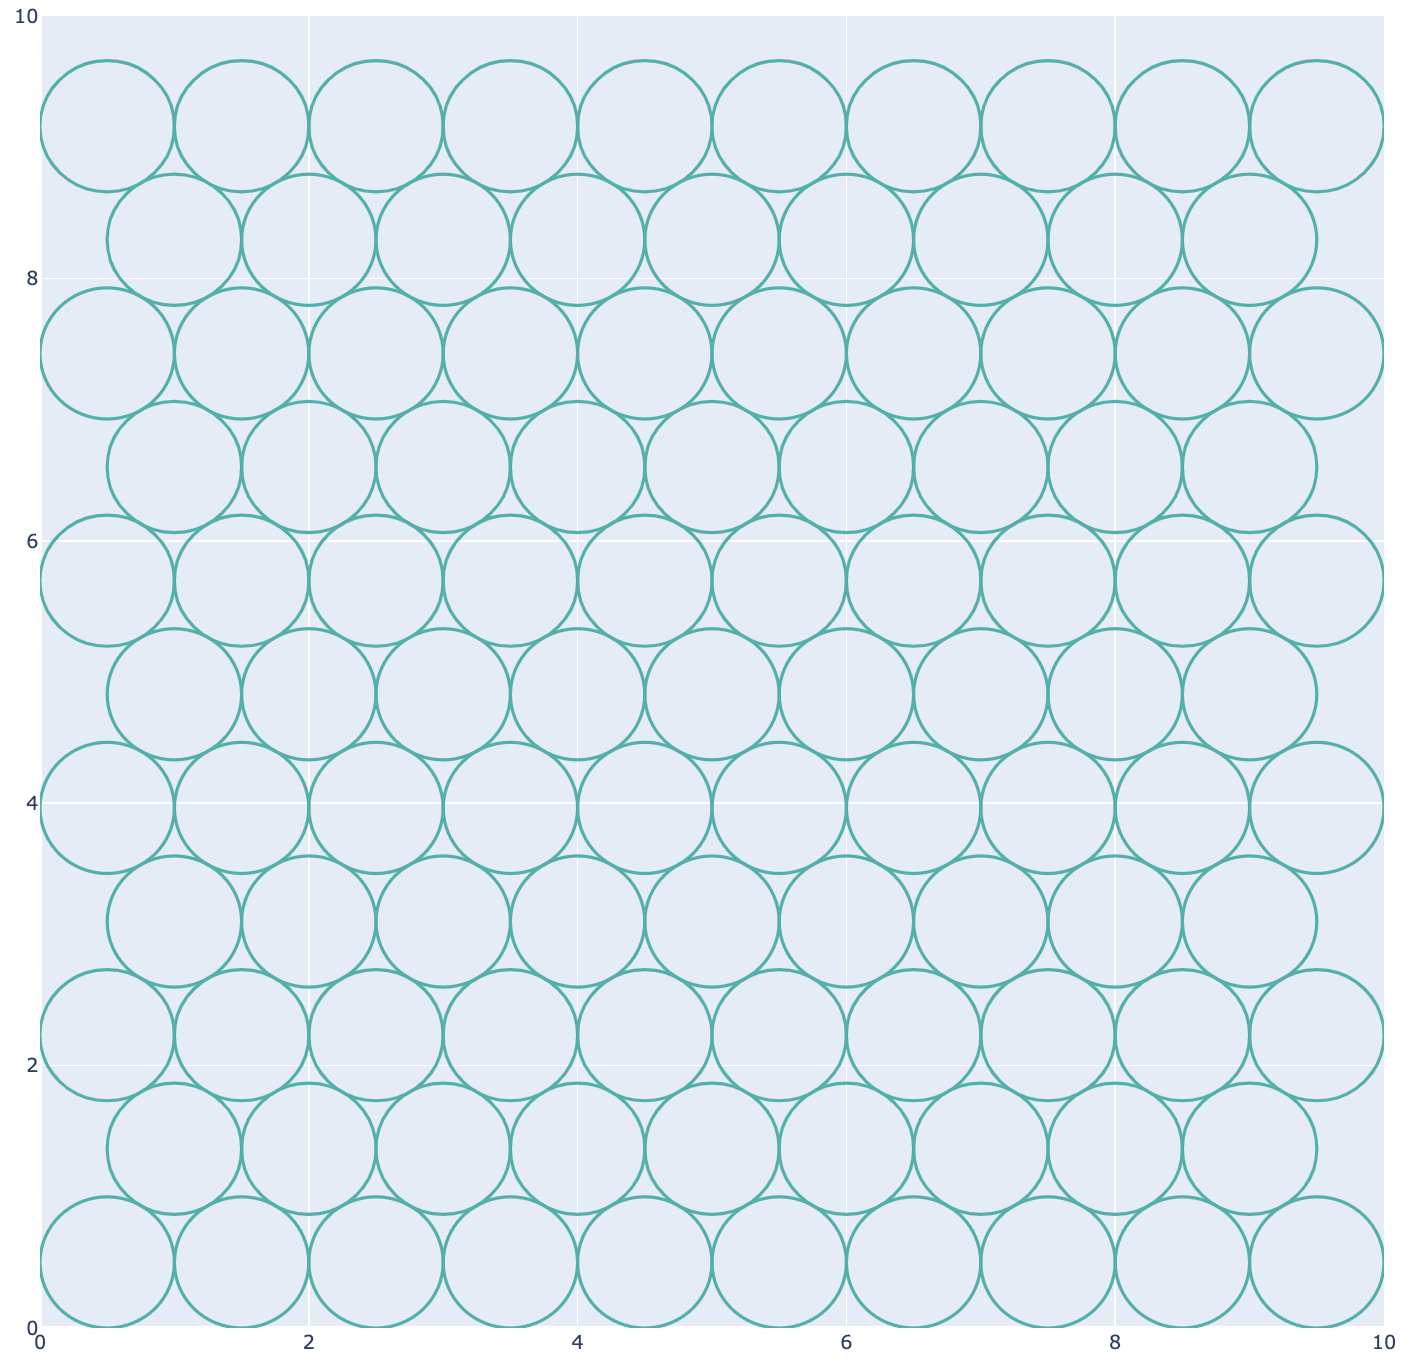
\includegraphics [width=\imgsize,height=\imgsize]
            {figures/\imgsubdir/105_packing.png}
            \caption{Шаров $105$, до перемешивания}
        \end{subfigure}
        \begin{subfigure}{0.49\textwidth}
            \centering
            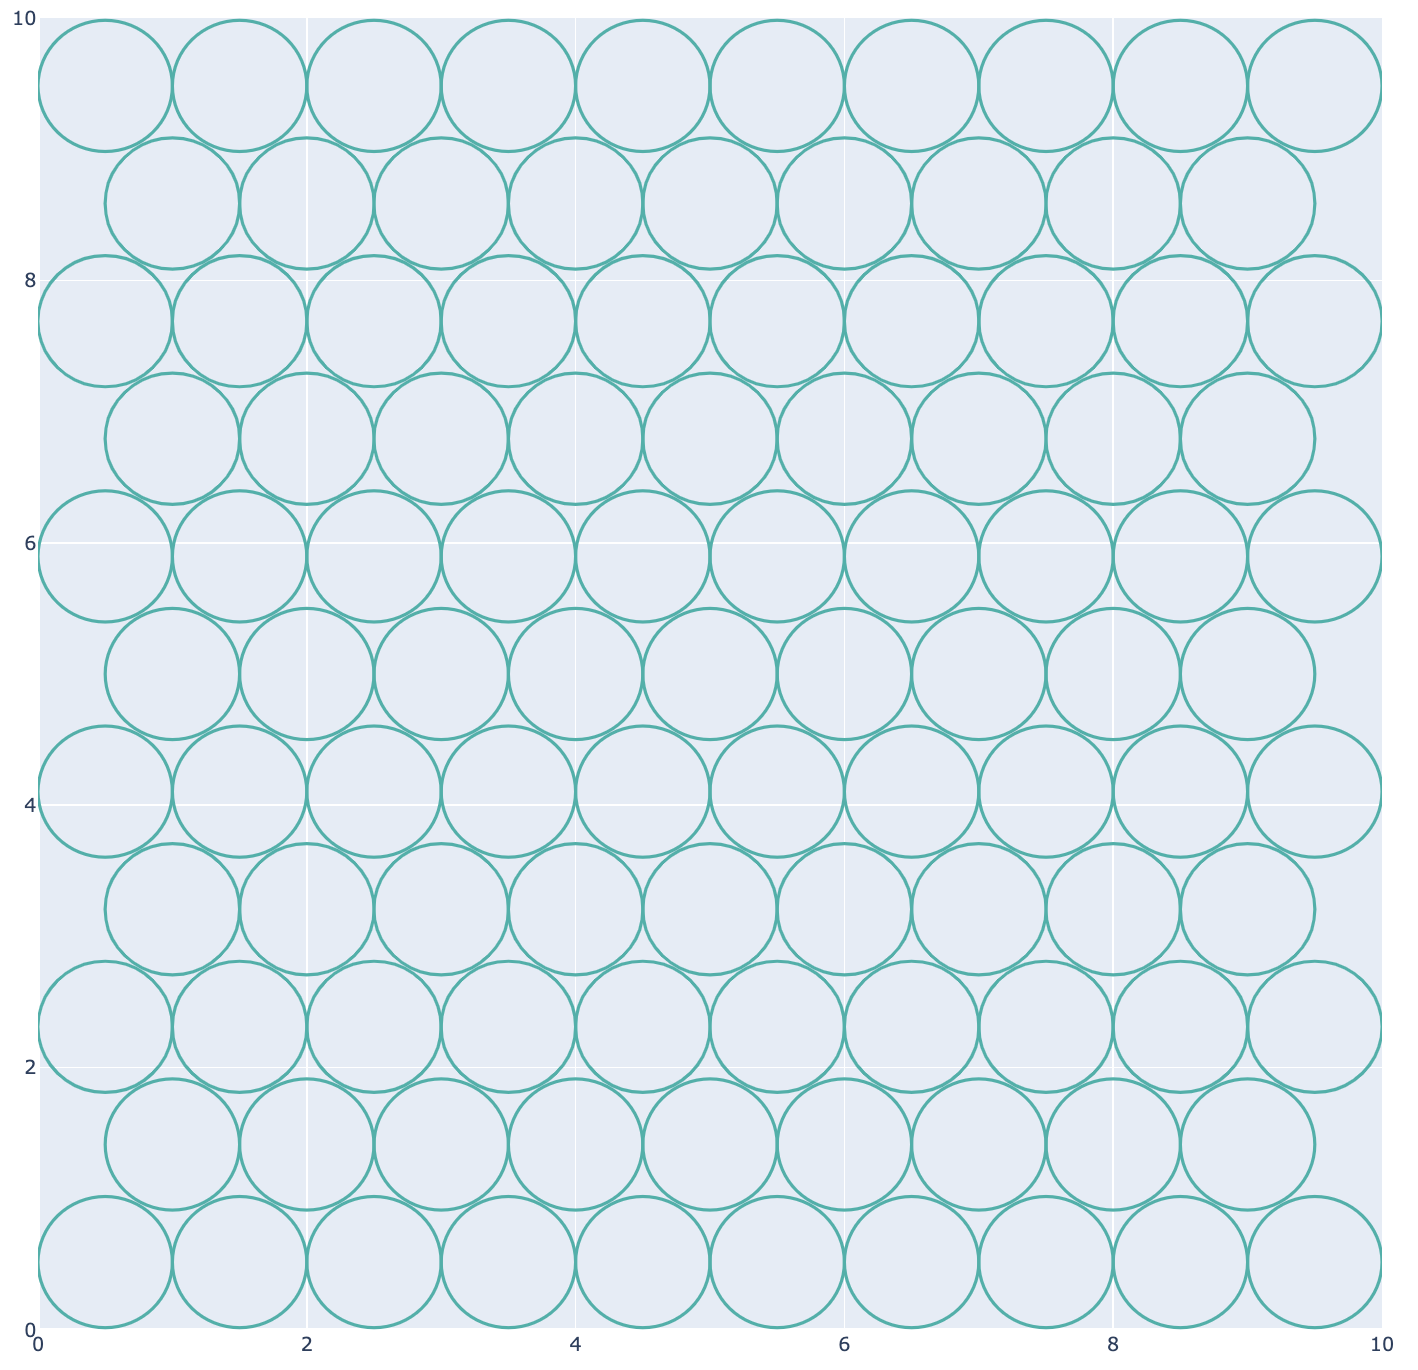
\includegraphics [width=\imgsize,height=\imgsize]
            {figures/\imgsubdir/105_shuffeling.png}
            \caption{Шаров $105$, после перемешивания}
        \end{subfigure}
        \caption{Расположение шаров}
        \label{fig:tight_packing}
    \end{figure}
    На изображениях \ref{fig:tight_packing} можно увидеть, что при расположении элементов в порядке плотнейшей упаковки можно добиться большей плотности. При том-же размере пространства при помощи плотнейшей упаковки вместо 81 сфер можно расположить до 105. 

\end{enumerate}

В результате тестов на максимальную плотность упаковки, алгоритмы основывающиеся на плотнейшей упаковке оказываются лучшими, поэтому для трёхмерный объектов также выбран метод плотнейших упаковок.

\newcommand{\imgsubdir}{tight_packing}
\begin{figure}[h!]
    \centering
    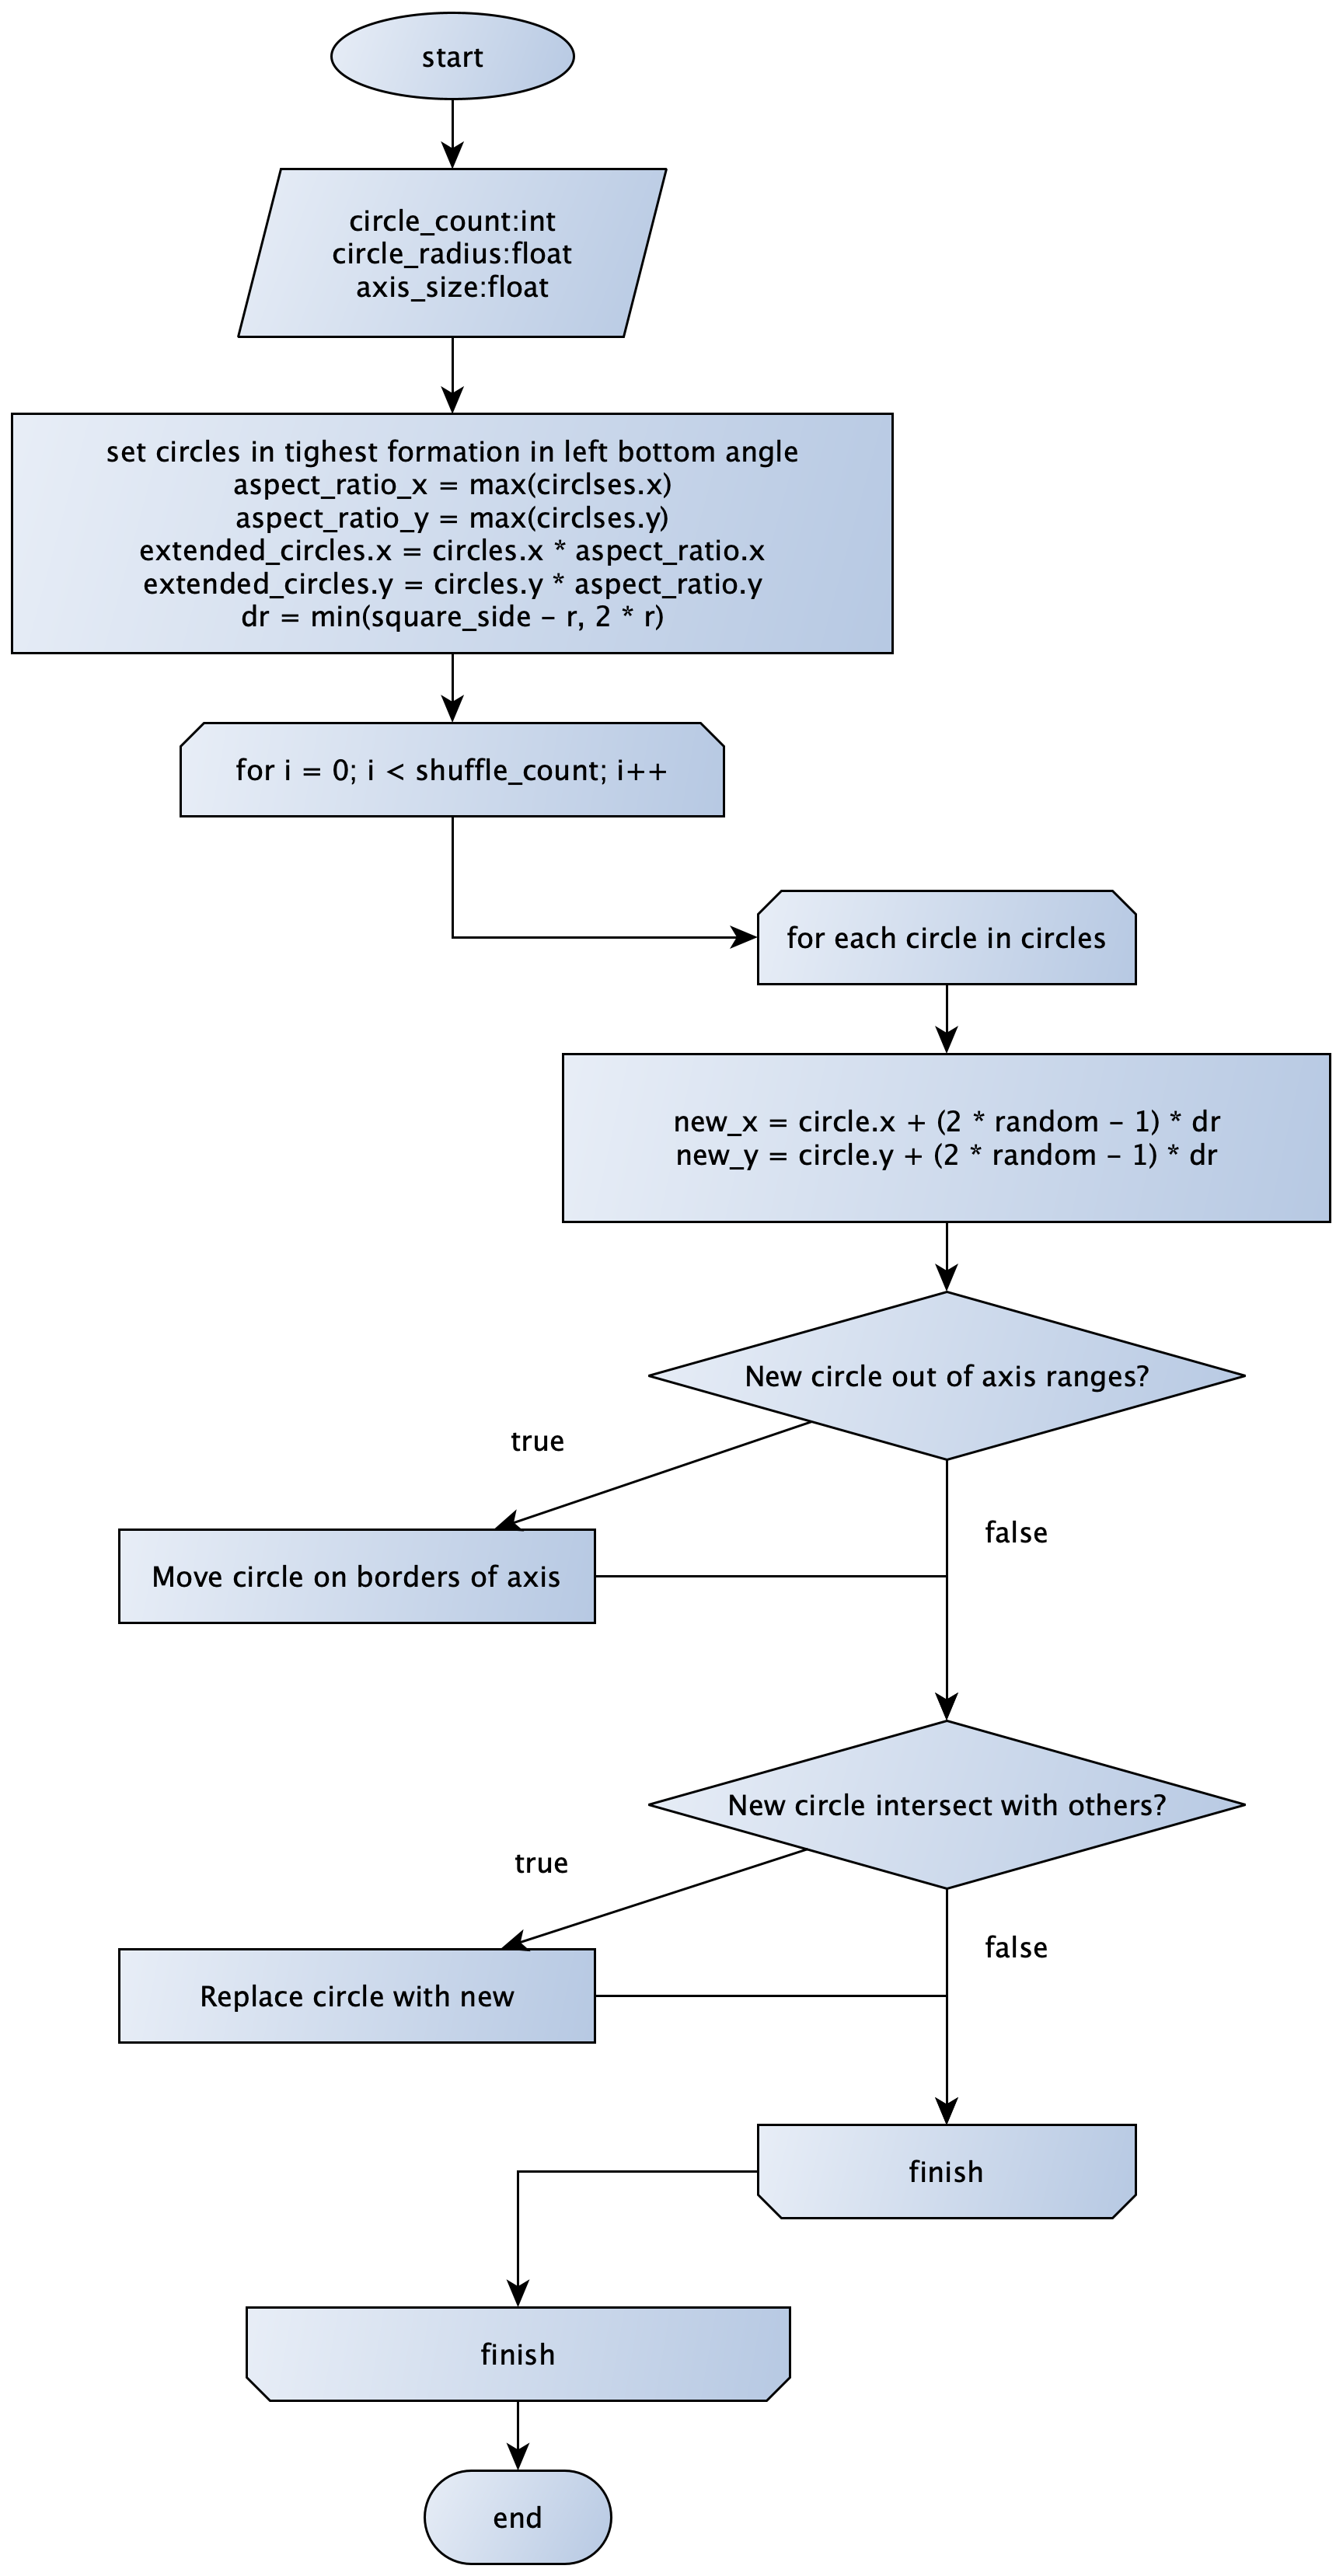
\includegraphics
    [width=15cm,height=20cm]
    {figures/\imgsubdir/block_scheme.png}
    \caption{Блок-схема расположения основанного на сетке}
    \label{fig:my_label}
\end{figure}
